\appendix
%\chapter{Notations utilis�es}
%
%\begin{itemize}
%\item{$N$ : le nombre d'agents,}
%\item{$\Act$ : l'ensemble des actions,}
%\item{$\JAct$ : l'ensemble des actions jointes,}
%\item{$\ca_i$ : la variable d'action de l'agent $i$,}
%\item{$\Xta$ : l'ensemble des variables d'�tat,}
%\item{$\ba$ : une action jointe,}
%\item{$\cx_k$ : une variable d'�tat $k$,}
%\item{$\Dom_k$ : le domaine de la variable $\cx_k$,}
%\item{$\Sta$ : l'ensemble des �tats,}
%\item{$\JSta$ : l'ensemble des �tats globaux joints,}
%\item{$\bs$ : un �tat global conjoint,}
%\item{$s_i$ : une instance des variables de l'agent $i$ ou l'�tat de l'agent $i$,}
%\item{$\Omega$ : l'ensemble des observations,}
%\item{$\JObs$ : l'ensemble des observations jointes,}
%\item{$\bo$ : une observation jointe,}
%\item{$o_i$ : l'observation de l'agent $i$,}
%\item{$\bo_{-i}$ : l'observation jointe de tous les agents sauf $i$,}
%\item{$\Tra$ : une fonction de transition,}
%\item{$\Tra_{ss'}^a = \Tra(s,a,s')$ : la probabilit� de transition de l'�tat $s$ � $s'$ par l'action $a$,}
%\item{$\Obs$ : une fonction d'observation,}
%\item{$\Obs_{ss'}^{a,o} = \Obs(o,s,a,s')$ : la probabilit� d'observation de $o$ lors de la transition de l'�tat $s$ � $s'$ par l'action $a$,}
%\item{$\Rew$ : une fonction de r�compense,}
%\item{$\Rew_s^a = \Rew(s,a)$ : la r�compense obtenue dans l'�tat $s$ apr�s avoir fait l'action $a$,}
%\end{itemize}

\chapter{Complexit� algorithmique des mod�les de Markov multiagents}
\label{anx:cplx}

\begin{summary}
Dans cette annexe une autre approche de la complexit� dans les processus de Markov multiagents � horizon fini est pr�sent�e selon les degr�s d'observabilit� de chacun des agents. Les mod�les les plus simples sont tout d'abord pr�sent�s, suivis ensuite par les mod�les les plus complexes. La complexit� algorithmique des mod�les monoagents n'est pas pr�cis�e dans cette annexe puisqu'elle reste identique � celle des mod�les multiagents dans la mesure o� le nombre d'agents est fix�.
\end{summary}

Les hypoth�ses classiques des mod�les de Markov stipulent qu'un groupe d'agents �volue \emph{simultan�ment} dans un environnement stochastique \emph{commun � tous}. � chaque �tape de temps discr�te, chacun des agents choisit une action � partir de sa politique locale, et l'ensemble des actions choisies constitue l'action jointe effectu�e dans l'environnement. Cette action jointe provoque la transition de l'environnement depuis l'�tat $s$ vers un �tat $s'$ d�termin� par la fonction de transition de l'environnement. Dans le cas partiellement observable, chacun des agents re�oit alors une observation de ce nouvel �tat, ou le nouvel �tat lui-m�me si l'environnement est compl�tement observable. Plus formellement, on peut rappeler qu'un processus de d�cision de Markov compl�tement observable est d�fini de la mani�re suivante:
\begin{definition}(\mmdp)
Un \mmdp est d�fini par un tuple $\la \alpha, \Sta, \{\Act_i\}_{i\in\alpha}, \Tra, \Rew, T \ra$, o�:
\begin{itemize}
\item  $\alpha$ est un ensemble fini d'\emph{agents} $i \in \alpha, 1 \leq i \leq n$;
\item $\Sta$ est un ensemble fini d'\emph{�tats} $s \in \Sta$;
\item $\Act_i$ est un ensemble fini d'\emph{actions} pour l'agent $i$ $a_i \in \Act_i$;
\item $\Tra(s,a_1,\ldots,a_n,s'): \Sta \times \JAct \times \Sta \mapsto [0,1]$ est la \emph{probabilit� de transition} du syst�me de l'�tat $s$ vers l'�tat $s'$ apr�s l'ex�cution de l'action jointe $\ba = \la a_1,\ldots,a_n,\ra$;
\item $\Rew(s,a_1,\ldots,a_n): \Sta \times \JAct\mapsto \mathds{R}$ est la \emph{r�compense} produite par le syst�me lorsque l'action  jointe $\ba$ est ex�cut�e dans l'�tat $s$;
\item $T$ est l'horizon de planification.
\end{itemize}
\end{definition}

Graphiquement, ce mod�le se repr�sente comme montr� par la figure~\ref{afig:mmdp} pour le cas � deux agents. Chacun des agents conna�t l'�tat � chaque �tape de d�cision et influence l'�tat suivant. Les r�compenses ont �t� omises pour des raisons de clart�.

\begin{figure}[h!tb]
\begin{center}
          \begin{tikzpicture}[scale=.7]%
        %\draw[step=1cm,color=gray,very thin] (-5,-1) grid (9,5);%%
        \filldraw[rounded corners,ultra thick,bleu] (-13,3) rectangle (6,1);%%
        \filldraw[rounded corners,ultra thick,vert] (-13,-3) rectangle (6,-1);%%
        \begin{scope}[shape=circle,inner sep=.02cm,fill=white]
        \tikzstyle{every node}=[draw,font=\footnotesize] %%
        \node (s0) at (-10,0)  {$\cs^0$}; %%
        \node (s1) at (-7,0)  {$\cs^1$}; %%
        \node (s2) at (-4,0)  {$\cs^2$}; %%
        \node (s3) at (-1,0)  {$\cs^3$}; %%
        \node (st) at (6,0)  {$\cs^T$}; %%
        \end{scope}
        \begin{scope}[shape=rectangle,inner sep=.05cm,fill=white]
        \tikzstyle{every node}=[draw,font=\small] %%
        \node (a11) at (-8,2)  {$\ca_1^1$}; %%
        \node (a21) at (-8,-2)  {$\ca_2^1$}; %%
        \node (a12) at (-5,2)  {$\ca_1^2$}; %%
        \node (a22) at (-5,-2)  {$\ca_2^2$}; %%
        \node (a13) at (-2,2)  {$\ca_1^3$}; %%
        \node (a23) at (-2,-2)  {$\ca_2^3$}; %%
        \node (a1t) at (4,2)  {$\ca_1^T$}; %%
        \node (a2t) at (4,-2)  {$\ca_2^T$}; %%
        \end{scope}
        \node[font=\small] at (-11,2)  {Agent 1}; %%
        \node[font=\small] at (-11,-2)  {Agent 2}; %%
        \draw[->,-latex] (s0)--(s1);  %%
        \draw[->,-latex] (a11)--(s1);  %%
        \draw[->,-latex] (a21)--(s1); %%
        \draw[->,-latex] (s1)--(s2); %%
        \draw[->,-latex] (a12)--(s2);  %%
        \draw[->,-latex] (a22)--(s2); %%
        \draw[->,-latex] (s2)--(s3); %%
        \draw[->,-latex] (a13)--(s3);  %%
        \draw[->,-latex] (a23)--(s3); %%
        \draw[->,-latex,densely dotted,thick] (s3)--(st); %%
        \draw[->,-latex] (a1t)--(st);  %%
        \draw[->,-latex] (a2t)--(st); %%
        \draw[->,-latex,dashed] (s0)--(a11); %%
        \draw[->,-latex,dashed] (s0)--(a21);  %%
        \draw[->,-latex,dashed] (s1)--(a12); %%
        \draw[->,-latex,dashed] (s1)--(a22);  %%
        \draw[->,-latex,dashed] (s2)--(a13); %%
        \draw[->,-latex,dashed] (s2)--(a23);  %%
        \draw[->,-latex,loosely dashed,thick] (s3)--(a1t); %%
        \draw[->,-latex,loosely dashed,thick] (s3)--(a2t);  %%
        \end{tikzpicture}%

  \caption{Probl�me de d�cision de Markov � deux agents et � horizon fini (\mmdp).\label{afig:mmdp}}
\end{center}
\end{figure}

D�s lors que les agents n'acc�dent plus directement � l'�tat mais seulement � une observation de celui-ci, le probl�me devient alors partiellement observable. Si tous les agents ont tout de m�me acc�s aux observations de tous les autres agents, le mod�le utilis� est un \pomdp multiagent ou \mpomdp:
\begin{definition}
 Un \mdp partiellement observable multiagent (\mpomdp) est d�fini par un tuple $\la \alpha, \Sta, \{\Act_i\}_{i\in\alpha}, \Tra,\{\Omega_i\}_{i\in\alpha},\Obs, \Rew, T \ra$, o�:%\\
\emph{\begin{itemize}
\item $\la \alpha, \Sta, \{\Act_i\}_{i\in\alpha}, \Tra, \Rew, T \ra$ est un \mmdp;%\\
\item $\Omega_i$  est l'ensemble fini des \emph{observations} de l'agent $i$ et $\JObs = \varprod_{i\in\alpha} \Omega_i$  est l'ensemble des observations jointe, o� $\bo = \la o_1,\ldots,o_n\ra \in \JObs$, $o_i \in \Omega_i$, est une observation jointe;%\\
\item $\Obs(\bo|\ba,s'): \Sta \times \JAct \times \JObs \mapsto [0,1]$ est la \emph{fonction d'observation} repr�sentant la probabilit� de recevoir l'observation jointe $\bo$ lors de la transition vers $s'$ sous l'effet de l'action jointe~$\ba$.
\end{itemize}}
\end{definition}

La figure~\ref{afig:mpomdp} repr�sente graphiquement un \mpomdp � deux agents � horizon fini. Chacun des agents conna�t l'observation re�ue par tous les autres agents � chaque �tape de d�cision. Comparativement � la figure~\ref{afig:mmdp}, les agents ne re�oivent qu'une information partielle � propos de l'�tat. Tous les agents peuvent toutefois maintenir la m�me distribution pour l'�tat de croyance puisqu'ils ont tous acc�s � toutes les observations. Finalement, dans le cas o� ils n'ont pr�cis�ment pas acc�s aux observations des autres agents, le mod�le devant �tre utilis� est un \decpomdp:
\begin{definition}
Un \pomdp d�centralis� (\decpomdp) est un tuple $\la\alpha,$ $\Sta,$ $\{\Act_i\}_{i\in\alpha},$ $\Tra,$ $\{\Omega_i\}_{i\in\alpha},$ $\Obs,$ $\Rew, T\ra$, o�:%\\
\emph{\begin{itemize}
\item $\la \alpha, \Sta, \{\Act_i\}_{i\in\alpha}, \Tra,\{\Omega_i\}_{i\in\alpha},\Obs, \Rew, T \ra$ est un \mpomdp;%\\
\item Chaque agent $i$ a uniquement acc�s � son propre historique $h_i^t$ des observations $o_i^1$ � $o^{t-1}_i$ pour prendre sa d�cision $a_i^t$ au temps $t$.
\end{itemize}}
\end{definition}
Dans le reste de cette annexe, nous supposerons que $\forall i, \Act_i = \Act$ et $\Omega_i = \Omega$ pour la simplicit� des explications.
\begin{figure}[h!tb]
\begin{center}
          \begin{tikzpicture}[scale=.7]%
        %\draw[step=1cm,color=gray,very thin] (-5,-1) grid (9,5);%%
        \filldraw[draw,rounded corners,ultra thick,bleu] (-13,3) rectangle (6,1);%%
        \filldraw[draw,rounded corners,ultra thick,vert] (-13,-3) rectangle (6,-1);%%
        \begin{scope}[shape=circle,inner sep=.02cm,fill=white]
        \tikzstyle{every node}=[draw,font=\footnotesize] %%
        \node (s0) at (-10,0)  {$\cs^0$}; %%
        \node (s1) at (-7,0)  {$\cs^1$}; %%
        \node (s2) at (-4,0)  {$\cs^2$}; %%
        \node (s3) at (-1,0)  {$\cs^3$}; %%
        \node (st) at (6,0)  {$\cs^T$}; %%
        \node (o11) at (-7,2)  {$\co_1^1$}; %%
        \node (o21) at (-7,-2)  {$\co_2^1$}; %%
        \node (o12) at (-4,2)  {$\co_1^2$}; %%
        \node (o22) at (-4,-2)  {$\co_2^2$}; %%
        \node (o13) at (-1,2)  {$\co_1^2$}; %%
        \node (o23) at (-1,-2)  {$\co_2^2$}; %%
        \end{scope}
        \begin{scope}[shape=rectangle,inner sep=.05cm,fill=white]
        \tikzstyle{every node}=[draw,font=\small] %%
        \node (a11) at (-8.5,2)  {$\ca_1^1$}; %%
        \node (a21) at (-8.5,-2)  {$\ca_2^1$}; %%
        \node (a12) at (-5.5,2)  {$\ca_1^2$}; %%
        \node (a22) at (-5.5,-2)  {$\ca_2^2$}; %%
        \node (a13) at (-2.5,2)  {$\ca_1^3$}; %%
        \node (a23) at (-2.5,-2)  {$\ca_2^3$}; %%
        \node (a1t) at (4,2)  {$\ca_1^T$}; %%
        \node (a2t) at (4,-2)  {$\ca_2^T$}; %%
        \end{scope}
        \node[font=\small] at (-11,2)  {Agent 1}; %%
        \node[font=\small] at (-11,-2)  {Agent 2}; %%
        \draw[->,-latex] (s0)--(s1);  %%
        \draw[->,-latex] (a11)--(s1);  %%
        \draw[->,-latex] (a21)--(s1); %%
        \draw[->,-latex] (s1)--(s2); %%
        \draw[->,-latex] (a12)--(s2);  %%
        \draw[->,-latex] (a22)--(s2); %%
        \draw[->,-latex] (s2)--(s3); %%
        \draw[->,-latex] (a13)--(s3);  %%
        \draw[->,-latex] (a23)--(s3); %%
        \draw[->,-latex,densely dotted,thick] (s3)--(st); %%
        \draw[->,-latex] (a1t)--(st);  %%
        \draw[->,-latex] (a2t)--(st); %%
        \draw[->,-latex] (a11)--(o11);  %%
        \draw[->,-latex] (a21)--(o21); %%
        \draw[->,-latex] (s1)--(o11);  %%
        \draw[->,-latex] (s1)--(o21); %%
        \draw[->,-latex] (a12)--(o12);  %%
        \draw[->,-latex] (a22)--(o22); %%
        \draw[->,-latex] (s2)--(o12);  %%
        \draw[->,-latex] (s2)--(o22); %%
        \draw[->,-latex] (a13)--(o13);  %%
        \draw[->,-latex] (a23)--(o23); %%
        \draw[->,-latex] (s3)--(o13);  %%
        \draw[->,-latex] (s3)--(o23); %%
%        \draw[->,-latex] (a1t)--(o1t);  %%
%        \draw[->,-latex] (a2t)--(o2t); %%
%        \draw[->,-latex] (st)--(o1t);  %%
%        \draw[->,-latex] (st)--(o2t); %%
        \draw[->,-latex,dashed] (o11)--(a12); %%
        \draw[->,-latex,dashed] (o21)--(a22);  %%
        \draw[->,-latex,dashed] (o12)--(a13); %%
        \draw[->,-latex,dashed] (o22)--(a23);  %%
        \draw[->,-latex,loosely dashed,thick] (o13)--(a1t); %%
        \draw[->,-latex,loosely dashed,thick] (o23)--(a2t);  %%
        \draw[->,-latex,dashed] (o21)--(a12); %%
        \draw[->,-latex,dashed] (o11)--(a22);  %%
        \draw[->,-latex,dashed] (o22)--(a13); %%
        \draw[->,-latex,dashed] (o12)--(a23);  %%
        \draw[->,-latex,loosely dashed,thick] (o23)--(a1t); %%
        \draw[->,-latex,loosely dashed,thick] (o13)--(a2t);  %%
        \draw[->,-latex,dashed] (a11)-- +(1,-2.5)--(a22); %%
        \draw[->,-latex,dashed] (a21)-- +(1,2.5)--(a12);  %%
        \draw[->,-latex,dashed] (a12)-- +(1,-2.5)--(a23); %%
        \draw[->,-latex,dashed] (a22)-- +(1,2.5)--(a13);  %%
        \draw[->,-latex,loosely dashed] (a13)-- +(1,-2.5)--(a2t); %%
        \draw[->,-latex,loosely dashed] (a23)-- +(1,2.5)--(a1t);  %%
        \end{tikzpicture}% 
  \caption{Probl�me de d�cision de Markov partiellement observable � deux agents et � horizon fini (\mpomdp).\label{afig:mpomdp}}
\end{center}
\end{figure}

La figure~\ref{afig:decpomdp} repr�sente graphiquement un \decpomdp � deux agents � horizon fini. Chacun des agents ne conna�t dans ce mod�le que son propre historique des observations et des actions repr�sent� par les cadres. Comparativement � la figure~\ref{afig:mpomdp}, les agents ne re�oivent plus aucune information quant � l'observation de l'autre agent ou � son action.
\begin{figure}[h!tb]
\begin{center}
  \input{a_decpomdp}
  \caption{Probl�me de d�cision de Markov partiellement observable d�centralis� � deux agents et � horizon fini (\decpomdp).\label{afig:decpomdp}}
\end{center}
\end{figure}

Comme nous l'avons expliqu� au chapitre~\ref{chap:2}, r�soudre un mod�le de Markov multiagent consiste � trouver une \emph{politique} pour chaque agent qui maximise l'\emph{utilit� esp�r�e} $EU$ (pour \emph{expected utility}) de tous les agents. Une politique est un ensemble de r�gles de d�cision, une pour chaque �tape de temps, qui associe l'historique des observations des agents � l'action jointe � effectuer dans l'environnement. Dans le cas compl�tement observable (\mmdp), puisque l'�tat est une statistique suffisante pour le choix de la meilleure action � effectuer selon la fonction de r�compense (Propri�t� de Markov), une politique associe simplement une action � tous les �tats accessibles � une �tape de temps. Pour r�sumer:
\begin{definition}\label{acplx:mmdpPolDef}
Dans le cas compl�tement observable,
\begin{itemize}
  \item Une \emph{r�gle de d�cision individuelle} $\delta_i^t$ pour l'agent $i$, est une association $\Sta \mapsto \Act$ pour chaque �tape $t$;
  \item Une \emph{r�gle de d�cision jointe} $\delta^t = \{\delta_i^t\}_{i\in \alpha}$ est une association $\Sta \mapsto \JAct$ pour chaque �tape~$t$;
  \item Une \emph{politique individuelle} $\Delta_i$ est une s�quence de $T$ r�gles de d�cisions individuelles, une pour chaque �tape;
  \item Une \emph{politique jointe} $\Delta = (\delta^1, ..., \delta^T) = \la \Delta_1, ..., \Delta_n\ra$ est une s�quence de $T$ r�gles de d�cisions jointes, une pour chaque �tape, ou bien un ensemble de politiques individuelles, une pour chaque agent.
\end{itemize}
\end{definition}

Cependant, dans le cas partiellement observable, les agents ne per�oivent l'�tat r�el du syst�me qu'au travers d'observations souvent bruit�es ou statistiquement insuffisantes. Chacun d'eux doit alors m�moriser la s�quence compl�te des observations per�ues (appel� l'historique) pour pouvoir agir de mani�re optimale. Une \emph{politique jointe} $\Delta$ � horizon $T$ est alors d�finie comme une s�quence de $T$ r�gles de d�cisions $\delta^t$ o� chaque $\delta^t$ associe un historique de longueur $t$ � une action jointe de $\JAct$:
\begin{definition}\label{acplx:decpomdpPolDef}
Dans le cas partiellement observable,
\begin{itemize}
  \item Une \emph{r�gle de d�cision individuelle} $\delta_i^t$ pour l'agent $i$, est une association $\mathcal{H}_i^t \mapsto \Act$ pour chaque �tape $t$;
  \item Une \emph{r�gle de d�cision jointe} $\delta^t = \{\delta_i^t\}_{i\in \alpha}$ est une association $\varprod_{i\in\alpha}\mathcal{H}_i^t \mapsto \JAct$ pour chaque �tape $t$;
  \item Une \emph{politique individuelle} $\Delta_i$ et une \emph{politique jointe} $\Delta$ sont identiques � celles de la d�finition~\ref{acplx:mmdpPolDef}.
\end{itemize}
O� $\mathcal{H}_i^t$ est l'ensemble des historiques $h_i^t = (o_i^1, ...,o_i^{t-1})$ � horizon $t$.
\end{definition}

Si l'on d�note par $w^T$ le \emph{monde} � horizon $T$ qui contient l'historique joint � horizon $T$ de toutes les observations et la s�quence -- possiblement non observable -- des �tats de l'environnement sur les $T$ �tapes de temps, on peut alors calculer la probabilit� de cette s�quence �tant donn� une politique $\Delta$:
\begin{equation}\label{aeq:prw}
\Pr\nolimits_\Delta(w^T) = \Pr(s^0) \prod_{t=1}^{T-1} \Obs(\bo^{t}|s^{t},\ba^{t}) \prod_{t=1}^T \Tra(s^{t}|s^{t-1},\ba^{t})
\end{equation}
O� $\ba^{t} = \delta^t(h^{t})$. Il convient de remarquer que dans les \mmdps $\Obs(\bo^{t}|s^{t},\ba^{t}) = 1$ si et seulement si $\forall i, o_i^t = s^t$.

La contribution � l'utilit� esp�r�e d'un monde � horizon $T$ est alors donn�e par:
\begin{equation}\label{aeq:euw}
eu_\Delta(w^T) = \Pr\nolimits_\Delta(w^T) \sum_{t=1}^{T} \Rew(s^{t},\ba^{t})
\end{equation}

Finalement, trouver une \emph{politique optimale} correspond � trouver une \emph{politique jointe} $\Delta$ qui maximise l'utilit� esp�r�e de tous les mondes possibles sur l'horizon $T$:
\begin{eqnarray}%\max_{\{\delta^t\}_{t=1}^T}
    EU(\Delta) &=& \sum_{\{s^t\}_{t=0}^T} \sum_{\{\bo^t\}_{t=1}^{T-1}} eu_\Delta(w^t) \\
    \mathrm{et donc }\Delta^{*} &=& \arg \max_{\{\delta^t\}_{t=1}^T} EU(\Delta) \label{aeq:EU}
\end{eqnarray}

D�crivons maintenant un exemple permettant d'aider � la compr�hension des concepts pr�c�dents et de la complexit� des algorithmes d�taill�s dans la suite de cette annexe.
\begin{description}
\item[Probl�me du tigre multiagent~\citep{NTYPM.03}:] D�crit au chapitre~\ref{chap:5} de cette th�se, ce probl�me repr�sente deux agents faisant face � deux portes. Derri�re l'une d'entre elles se trouve un tigre f�roce (associ� d'une grosse p�nalit�). Derri�re l'autre se trouve un tr�sor fabuleux (la r�compense). Chacun des agents peut ouvrir l'une ou l'autre des portes (par une action $o_\textsc{r}$ ou $o_\textsc{l}$ pour \emph{open right} et \emph{open left}) ou se contenter d'�couter ($\textsc{l}is$ pour \emph{listen}). Lorsqu'un agent �coute, une petite p�nalit� est inflig�e et l'agent qui �coute re�oit une observation bruit�e de l� o� se situe le tigre ($\textsc{r}$ ou $\textsc{l}$ pour \emph{right} et \emph{left}). D�s qu'un des agents tente d'ouvrir une porte, le monde est r�initialis�, repla�ant le tigre derri�re l'une des portes al�atoirement. Les deux agents ont $T$ �tapes de temps pour maximiser leur utilit�. Le probl�me contient donc deux �tats -- $\textsc{r}$\emph{ight} et $\textsc{l}$\emph{eft}--, trois actions -- $o_\textsc{r},o_\textsc{l}$ et $\textsc{l}is$ -- et deux observations par agent -- $\textsc{r}$ et $\textsc{l}$ --. Il peut �tre factoris� en utilisant une variable d'�tat $\cs$ avec $\Sta = \{\textsc{r},\textsc{l}\}$, deux variables de d�cision $\ca_1$ et $\ca_2$ avec $\Act = \{o_\textsc{r},o_\textsc{l},\textsc{l}is\}$ et deux variables d'observation $\co_1$ et $\co_2$ avec $\Omega = \{\textsc{r},\textsc{l}\}$ par �tape de temps.
\end{description}
La figure~\ref{afig:decpomdp} donne une repr�sentation graphique de l'exemple pour $T$ �tapes de temps.

Une politique jointe peut aussi �tre repr�sent�e par un \emph{arbre de d�cision} o� les n\oe uds sont �tiquet�s par des actions et les arcs par des observations. Pour ex�cuter un arbre de politique, chaque agent commence � la racine de l'arbre, effectue l'action correspondante, suit la branche de l'arbre �tiquet�e par l'observation re�ue, et r�p�te le processus jusqu'� atteindre l'horizon final. Un exemple de politique � horizon 3 est donn� dans le cas du \mpomdp, i.e que les agents partagent leurs actions et observations. Cette politique consiste � �couter deux fois avant de choisir quelle porte ouvrir ou de r��couter si les agents ont re�u une information contradictoire quant � la position du tigre. Cet exemple est donn� par la figure~\ref{afig:treetiger}. Selon l'�quation~\eqref{aeq:EU}, il est possible d'�crire:
\begin{equation}\label{aeq:dectreehard}
    EU(\Delta^{*}) = \max_{\delta^1(h^1),\delta^2(h^2),\delta^3(h^3)} \sum_{\{s^t\}_{t=0}^3} \sum_{\bo^1,\bo^2} eu_\Delta(w^3)
\end{equation}
O� le monde $w^3$ correspond � une assignation des variables $(s^0,s^1,s^2,s^3,\bo^1,\bo^2)$.

Puisqu'au temps de d�cision $\ba^3 = \delta^3(\bo^1,\bo^2)$ les agents on d�j� observ� $\bo^1$ et $\bo^2$ et effectu� les actions $\ba^1$ et $\ba^2$, en utilisant la r�gle alg�brique suivante:
\begin{equation}\label{aeq:trans}
\mbox{If } \pi_x: \mathcal{Y}\mapsto\mathcal{X} \mbox{ alors } \max_{\pi_x} \sum_{y\in\mathcal{Y}}  f(\pi_x(y),y) = \sum_{y\in\mathcal{Y}}\max_{x\in\mathcal{X}} f(x,y)
\end{equation}
Il est possible de transformer l'�quation~\eqref{aeq:dectreehard},en:
\begin{equation}
      \eqref{aeq:dectreehard} \Leftrightarrow EU(\Delta^{*}) = \max_{\ba^1} \sum_{\bo^1} \max_{\ba^2} \sum_{\bo^2}\max_{\ba^3} \sum_{\{s^t\}_{t=0}^3} eu_\Delta(w^3)\label{dectree}
\end{equation}
La r�gle~\ref{aeq:trans} mod�le simplement le fait qu'� l'�tape de l'application de la fonction $\pi_x$, la valeur de la variable $y$ est connue et la maximisation est donc r�alis�e seulement sur les valeurs possibles de $x$ plut�t que sur toutes les associations possibles $\mathcal{Y}\mapsto\mathcal{X}$, assurant ainsi un gain exponentiel dans la complexit� en pire cas. L'int�r�t de telles transformations sera explicit� un peu plus loin dans cette annexe.

\begin{figure}[thb]\centering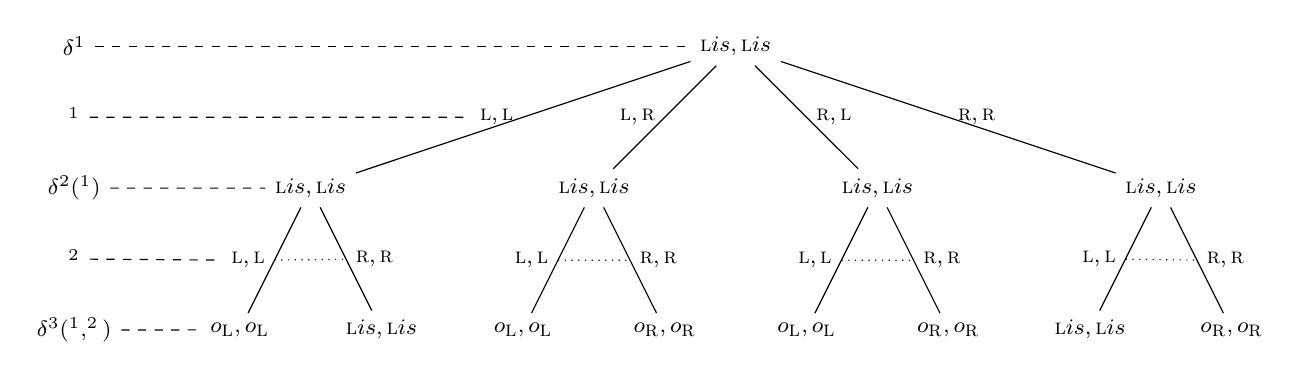
\begin{tikzpicture}[line width=.1ex, scale=1.2]
\tikzstyle{every node}=[font=\footnotesize] %%
\tikzstyle{level 1}=[sibling distance=3cm]
\tikzstyle{level 2}=[sibling distance=1.5cm]
\tikzstyle{level 3}=[sibling distance=.5cm]
\node (d1) at (0,0){$\delta^1$};%%
\node (o1) at (0,-.75){$\bo^1$};%%
\node (d2) at (0,-1.5){$\delta^2(\bo^1)$};%%
\node (o2) at (0,-2.25){$\bo^2$};%%
\node (d3) at (0,-3){$\delta^3(\bo^1,\bo^2)$};%%
\node (ld1) at (7,0) {$\la\textsc{l}is, \textsc{l}is\ra$}
   child {
            node (ld2) {$\la\textsc{l}is, \textsc{l}is\ra$}
            child {
                node(ld3) {$\la o_\textsc{l}, o_\textsc{l}\ra$}
                edge from parent
                node[left](1) {$\la \textsc{l}, \textsc{l}\ra$}
            }
            child {
                node {$\la\textsc{l}is, \textsc{l}is\ra$}
                edge from parent
                node[right](2) {$\la \textsc{r}, \textsc{r}\ra$}
            }
            edge from parent
            node[left] (lo1) {$\la \textsc{l}, \textsc{l}\ra$}
        }
    child {
            node {$\la\textsc{l}is, \textsc{l}is\ra$}
            child {
                node {$\la o_\textsc{l}, o_\textsc{l}\ra$}
                edge from parent
                node[left](3) {$\la \textsc{l}, \textsc{l}\ra$}
            }
            child {
                node {$\la o_\textsc{r}, o_\textsc{r}\ra$}
                edge from parent
                node[right](4) {$\la \textsc{r}, \textsc{r}\ra$}
            }
            edge from parent
            node[left] {$\la \textsc{l}, \textsc{r}\ra$}
        }
    child {
            node {$\la\textsc{l}is, \textsc{l}is\ra$}
            child {
                node {$\la o_\textsc{l}, o_\textsc{l}\ra$}
                edge from parent
                node[left](5) {$\la \textsc{l}, \textsc{l}\ra$}
            }
            child {
                node {$\la o_\textsc{r}, o_\textsc{r}\ra$}
                edge from parent
                node[right](6) {$\la \textsc{r}, \textsc{r}\ra$}
            }
            edge from parent
            node[right] {$\la \textsc{r}, \textsc{l}\ra$}
        }
    child {
            node {$\la\textsc{l}is, \textsc{l}is\ra$}
            child {
                node {$\la\textsc{l}is, \textsc{l}is\ra$}
                edge from parent
                node[left](7) {$\la \textsc{l}, \textsc{l}\ra$}
            }
            child {
                node {$\la o_\textsc{r}, o_\textsc{r}\ra$}
                edge from parent
                node[right](8) {$\la \textsc{r}, \textsc{r}\ra$}
            }
            edge from parent
            node[right] {$\la \textsc{r}, \textsc{r}\ra$}
   };
\draw[dotted] (1)--(2);
\draw[dotted] (3)--(4);
\draw[dotted] (5)--(6);
\draw[dotted] (7)--(8);
\draw[dashed] (d1)--(ld1);
\draw[dashed] (d2)--(ld2);
\draw[dashed] (d3)--(ld3);
\draw[dashed] (o1)--(lo1);
\draw[dashed] (o2)--(1);
\end{tikzpicture}
\caption{Exemple d'arbre de politique � horizon 3 dans le probl�me du tigre.}\label{afig:treetiger}
\end{figure}

\section{Comprendre les mod�les de Markov via l'alg�bre}\label{sect:unimarkov}

Voyons maintenant les cons�quences sur la complexit� en pire cas de l'ignorance des valeurs pass�es de toutes les variables de l'environnement au travers de l'�tude de l'�quation de l'utilit� esp�r�e d�crite par l'�quation~\eqref{aeq:EU}.

\subsection{\pac{mmdp}}
Dans les \mmdps, puisqu'il n'existe pas d'observation explicite, l'expression de la contribution � l'utilit� esp�r�e devient:
\begin{eqnarray}
    \eqref{aeq:euw}\Rightarrow eu_\Delta(w^T) &=& \Pr(s^0) \prod_{t=1}^{T} \Tra(s^{t}|s^{t-1},\ba^{t}) \sum_{t=1}^{T} \Rew(s^{t},\ba^{t})\notag\\
    \eqref{aeq:EU}\Rightarrow EU(\Delta^*) &=& \max_{\{\delta^t\}_{t=1}^T} \sum_{\{s^t\}_{t=0}^T} eu_\Delta(w^T)\label{aeq:EUmm}
\end{eqnarray}
O� $w^t = (s^0,...,s^{t-1})$.

La figure~\ref{afig:mmdp} montre une repr�sentation graphique d'un \mmdp � horizon $T$. Il convient de remarquer ici que bien que les �tats ne fassent pas partie de la connaissance des agents initialement, ils deviennent totalement observables au travers des liens d'informations. En consid�rant ce fait, il est �galement possible d'observer qu'au cours du temps, les agents ont effectivement acc�s � toutes les valeurs des variables de l'environnement. L'�quation~\eqref{aeq:EUmm} peut �tre alors transform�e en utilisant la r�gle~\eqref{aeq:trans}:
\begin{equation}
    \eqref{aeq:EUmm}\Leftrightarrow EU(\Delta^*) =\sum_{s^0}\max_{\ba^1}\sum_{s^1}...\max_{\ba^T}\sum_{s^T} eu_\Delta(w^T)\label{aeq:EUmms}
\end{equation}
O� $\ba^1 = \delta^1(s^0)$, $\ba^2 = \delta^2(s^0,s^1)$, etc.

\subsection{\pac{mpomdp}}
Dans les \mpomdps, puisque les agents n'ont pas acc�s � l'�tat r�el du monde, l'historique entier des actions et des observations pass�es doit �tre maintenu~\citep{SS.73}. Dans ce cas, l'expression de l'utilit� esp�r�e devient:
\begin{eqnarray}
\eqref{aeq:EU}\Rightarrow EU(\Delta^*) &=& \max_{\{\delta^t\}_{t=1}^T} \sum_{\{s^t\}_{t=0}^T} \sum_{\{\bo^t\}_{t=1}^{T-1}} eu_\Delta(w^T)\label{aeq:EUmpomdp}
\end{eqnarray}

La figure~\ref{afig:mpomdp} montre une repr�sentation graphique d'un \mpomdp � horizon $T$. Les liens d'information montrent que les agents ont acc�s � l'ensemble de l'historique des actions et des observations de l'autre agent (mais pas � l'�tat) et peuvent donc raisonner sur la m�me information. On observe alors que le nombre de transformations possibles dans l'�quation de l'utilit� esp�r�e est moindre; ainsi, de la m�me mani�re que nous avons transform� l'�quation~\eqref{aeq:EUmm} en l'�quation ~\eqref{aeq:EUmms}, il est possible de transformer l'�quation~\eqref{aeq:EUmpomdp} par l'application de la r�gle~\eqref{aeq:trans}:
\begin{equation}
    \eqref{aeq:EUmpomdp}\Leftrightarrow EU(\Delta^*) =\max_{\ba^1}\sum_{\bo^1}...\max_{\ba^T} \sum_{s^0,...,s^T} eu_\Delta(w^T) \label{aeq:EUpos}
\end{equation}
Il convient alors de remarquer que la derni�re somme sur les �tats possibles ne peut �tre distribu�e de la m�me mani�re que la somme sur les observations puisque les agents n'ont pas acc�s � la valeur r�elle de ces �tats pass�s au moment d'effectuer les d�cisions et doivent donc maintenir un \emph{�tat de croyance}. Cette croyance est repr�sent�e explicitement par la s�quence des observations re�ues depuis le d�but, ou peut �tre maintenue implicitement au travers d'une \emph{distribution de probabilit� sur les �tats} par l'utilisation de la r�gle de Bayes:
\[\bel^{t+1}(s') \propto \Obs(\bo|\ba,s') \int \Tra(s'|s,\ba) \bel^t(s)\,\mathrm{d}s\]
O� $\bel^{t} \in \Delta\Sta$ est une distribution de probabilit� sur le simplex sur $\Sta$ est est appel� \emph{�tat de croyance}.

\subsection{\pac{dec-pomdp}}
Bien plus complexes, les \decpomdps font l'hypoth�se que les agents n'ont pas acc�s � l'historique des autres agents. Chaque agent doit alors maintenir un \emph{�tat de croyance sur tous les historiques possibles des autres agents} et les transformations faites ci-avant sur l'�quation de l'utilit� esp�r�e ne fonctionnent plus. La figure~\ref{afig:decpomdp} montre une repr�sentation graphique d'un \decpomdp � horizon $T$. Par comparaison aux figures pr�c�dentes, il existe beaucoup moins de liens d'informations et les agents n'ont donc pas acc�s � l'observation ni � l'action des autres agents.

L'utilit� esp�r�e d'un \decpomdp est originalement la m�me que celle d'un \mpomdp (�quation~\eqref{aeq:EUmpomdp}). Cependant, puisque les simplifications ne s'appliquent pas � cause des connaissances partielles des agents. il est seulement possible de d�composer chaque politique jointe et chaque observation jointe pour chaque agent. Par exemple, si l'on consid�re seulement l'agent 1, la r�gle~\eqref{aeq:trans} peut �tre appliqu�e sur les d�cisions de l'agent 1:
\begin{eqnarray}
    EU(\Delta^*) &=& \max_{\delta^1,...,\delta^T} \sum_{s^0,...,s^T} \sum_{\bo^1,...,\bo^T} eu_\Delta(w^T) \notag\\
    &=& \max_{\{\delta_i^1,...,\delta_i^T\}_{i=1}^n} \sum_{\{o_i^1,...,o_i^{T-1}\}_{i=1}^n} \sum_{s^0,...,s^T} eu_\Delta(w^T) \notag\\
    &=& \max_{\{\delta_i^1,...,\delta_i^T\}_{i=2}^n}  \max_{a_1^1}\sum_{o_1^1}...\max_{a_1^{T-1}}\sum_{o_1^{T-1}}\max_{a_1^T}
    %\notag \\&&
    \sum_{\{o_i^1,...,o_i^{T-1}\}_{i=2}^n} \sum_{s^0,...,s^T} eu_\Delta(w^T) \label{aeq:EUdec2}
\end{eqnarray}
Cette derni�re �quation~\eqref{aeq:EUdec2} repr�sente � la fois que l'agent 1 doit raisonner sur un \emph{�tat de croyance} -- au travers de la somme sur les �tats -- et sur un \emph{�tat de croyance multiagent} qui consiste en toutes les politiques possibles de tous les autres agents consid�rant tous les historiques possibles d'observations. Un �tat de croyance multiagent peut aussi �tre vu comme un point dans le simplex sur $\Sta \times Q_{\neq i}^T$, o� $Q_{\neq i}^T$ repr�sente l'ensemble de toutes les politiques jointes � horizon $T$ pour tous les agents sauf $i$.

Voyons maintenant la complexit� algorithmique de ces mod�les � partir de la repr�sentation alg�brique de leur utilit� esp�r�e.

\section{Complexit� algorithmique des mod�les de Markov}\label{sect:cplxmarkov}

Pour cela consid�rons deux types d'algorithmes diff�rents: un qui met � profit l'espace m�moire pour am�liorer les temps de calcul et un autre qui, au contraire, �conomise la m�moire au d�triment du temps de calcul.

\subsection{Variable Elimination (\pac{ve})}

Le premier type algorithme consid�r� pour r�soudre ces probl�mes de Markov multiagents et l'algorithme par �limination de variable (\textsc{ve}~\citep{D.99}). Le principe de \textsc{ve} est d'utiliser la structure alg�brique du probl�me pour calculer l'utilit� esp�r�e globale en ne faisant que des calculs locaux du type de la programmation dynamique.

Par exemple, consid�rons trois fonctions $f(x,y), f(x,z), f(x,u)$ et supposons que l'on veut calculer $C = \max_{x,y,z,u} (f(x,y) + f(x,z) + f(x,u))$. Le principe de \textsc{ve} est d'\emph{�liminer} chaque variable successivement. �liminer $z$ consiste d'abord � d�composer $C$ comme
$C = \max_{x,y,u} (f(x,y)+(\max_z f(x,z))+ f(x,u))$. De fait, $z$ est �limin� en consid�rant seulement les fonctions locales qui d�pendent de $z$. Cela cr�e ainsi une nouvelle fonction $g(x)=\max_z f(x,z)$ qui ne d�pend que de $x$. Les autres variables peuvent ensuite �tre �limin�es de mani�re similaire pour obtenir la valeur de $C$. Les valeurs optimales de chacune des variables peuvent �tre m�moris�es pendant les calculs.

Plus g�n�ralement, \textsc{ve} peut �tre utilis� pour calculer l'�limination de variable sur une combinaison de fonctions, i.e sur des quantit�s de la forme $\mathop{\oplus}_V ( \otimes_{f \in F} f )$, o� $V$ est l'ensemble des variables � �liminer, $F$ est l'ensemble des fonctions locales (chacune des fonctions d�pendant d'un sous-ensemble de $V$), et $\oplus$ et $\otimes$ sont des op�rateurs satisfaisant les propri�t�s alg�briques telles que la commutativit�, l'associativit� ou la distributivit� de $\oplus$ sur $\otimes$. Il est �galement possible d'adapter \textsc{ve} � des cas incorporant plusieurs op�rateurs d'�limination et de combinaison~\citep{N.94}. Cette adaptation est requise pour les mod�les de Markov qui impliquent l'op�rateur d'�limination $\max$ sur les r�gles de d�cision et $\sum$ sur les �tats et les observations (cf. e.g. �quation~\eqref{aeq:dectreehard}), et l'op�rateur de combinaison $\times$ pour les probabilit�s conditionnelles et $\sum$ pour les r�compenses.

La complexit� temporelle et spatiale de \textsc{ve} est $O(|F|d^{\omega+1})$, o�:
\begin{itemize}
\item $|F|$ est le nombre de fonctions locales;
\item $d$ est la taille maximum des domaines des variables � �liminer;
\item $\omega$ est la \emph{taille induite par l'ordre d'�limination}. Ce param�tre est le nombre maximal de variables impliqu�es dans une fonction cr��e pendant les �liminations. Certains ordres d'�limination sont meilleurs que d'autres: dans l'exemple consid�r� ci-dessus, la taille induite par l'ordre d'�limination $z,y,x,u$ est de $1$ alors que que celle induite par l'ordre $x,y,z,u$ est de $3$. Si $\omega$ est la taille minimum induite quelque soit l'ordre d'�limination, il est simplement appel� \emph{taille induite}. Le trouver est g�n�ralement un probl�me \textsc{np}-complet~\citep{D.99}.
\end{itemize}

Lorsque plusieurs op�rateurs d'�limination sont impliqu�s, la complexit� th�orique n'est pas exponentielle dans la taille induite mais dans la \emph{taille induite contrainte}~\citep{PD.04,PSV.06b}, qui prend en compte le fait que la pr�sence de plusieurs op�rateurs d'�limination impose g�n�ralement des contraintes sur l'ordre d'�limination.

Pour \textsc{ve}, l'int�r�t principal de la transformation de quantit� de la forme \[(a)~\max_{\pi_x} \sum_{y} f(\pi_x(y),y) \mbox{ vers } (b)~\sum_{y} \max_x f(x,y)\] est de diminuer la taille du plus grand domaine des variables. Plus pr�cis�ment, dans $(a)$, la r�gle de d�cision $\pi_x$ peut �tre consid�r�e comme une variable dont le domaine est l'ensemble des tuples $E = \{(x_1,\ldots, x_{dom(y)|}),|,x_i \in dom(x)\}$. Chaque �l�ment de $E$ d�finit la valeur prise par $\pi_x$ pour chaque valeur de $y$. La taille de $E$ est donc de $|dom(x)|^{|dom(y)|}$. Pour $(b)$, la taille du plus grand domaine impliqu� est seulement de $\max( |dom(x)| , |dom(y)|)$, qui n'est pas exponentiel en $|dom(y)|$. Cela montre l'int�r�t de l'utilisation de la r�gle~\eqref{aeq:trans} pour la transformation des �quations~\eqref{aeq:EUmm} et~\eqref{aeq:EUmpomdp} en de nouvelles �quations~\eqref{aeq:EUmms}, \eqref{aeq:EUpos} et~\eqref{aeq:EUdec2}.

Il convient toutefois de remarquer que de telles transformations ne sont pas toujours possibles. Par exemple, \[\max\limits_{\pi_x , \pi_t} \sum_{y,z}  f(\pi_x(y),y , z , \pi_t(z))\] peut possiblement �tre transform�e en \[\max_{\pi_t} \sum_{y} \max_x \sum_{z} f(x,y , z , \pi_t(z)),\] mais pas dans une forme n'impliquant aucune �limination de r�gle de d�cision. Une telle situation appara�t g�n�ralement un premier agent conna�t seulement la valeur de la variable $y$ avant de prendre la d�cision $x$, tandis qu'un autre agent ne conna�t que la valeur de $z$ avant de prendre la d�cision $t$.

\subsection{Recherche dans un arbre}

� l'inverse de l'algorithme \textsc{ve}, la recherche dans un arbre est une m�thode de haut en bas qui cherche exhaustivement une solution optimale sur toutes les instanciations possibles des variables.

l'id�e principale de cet algorithme est d'instancier les variables et de calculer la valeur de chaque s�quence de d�cisions consid�rant tous les mondes possibles. L'algorithme~\ref{aalg:dfs} est un algorithme de recherche en profondeur d'abord (\textsc{dfs} pour \emph{Depth First Search}) qui explore r�cursivement toutes les assignations possibles des n\oe uds. Selon le type de n\oe ud, \textsc{dfs} choisira de maximiser (pour les n\oe uds de d�cision -- ligne~\ref{aalg:dfs:decnode}) ou de sommer (pour les n\oe uds d'observations ou d'�tats -- ligne~\ref{aalg:dfs:chnode}) les valeurs esp�r�es des diff�rentes instanciations de chacun des n\oe uds fils. D�s qu'il rencontre un n\oe ud feuille (une r�compense -- ligne~\ref{aalg:dfs:rewnode}), \textsc{dfs} calcule la valeur esp�r�e $eu_{\Delta_A}(w^T_A)$ �tant donn� l'instanciation $A$ correspondant au chemin parcouru depuis la racine jusqu'� la feuille.

\begin{algorithm}[h!tb]
\caption{Depth First Search (\textsc{dfs})\label{aalg:dfs}}
\begin{algorithmic}[1]
%\small
\algrenewcommand\alglinenumber{\tiny}
%\vspace{1mm}
%\Function{dfs}{$nL$, $A$}
\State{\textbf{Entr�e:} $L$: Une liste ordonn�e de n\oe uds}
\State{\phantom{\textbf{Entr�e:}}$A$: Une assignation des n\oe uds qui ne sont pas dans $L$}
\State{\textbf{Retourne:} La valeur esp�r�e maximale $EU(\Delta^*)$}
\State{$n \gets first(L)$}
\If{$n$ est un n\oe ud de d�cision\label{aalg:dfs:decnode}}
    \State{$val \leftarrow -\infty$}
    \ForAll{$v \in domain(n)$}
        \State{$val \gets \max(val,$\Call{dfs}{$queue(L)$,$A\cup\{n\gets v\}$}$)$}
    \EndFor
    \State{\Return{$val$}}
\EndIf
\If{$n$ est un n\oe ud d'observation ou d'�tat\label{aalg:dfs:chnode}}
    \State{$val \gets 0$}
    \ForAll{$v \in domain(n)$}
        \State{$val \gets val+$\Call{dfs}{$queue(L)$, $A\cup\{n\gets v\}$}}
    \EndFor
    \State{\Return{$val$}}
\EndIf
\State{\textbf{Si} $n$ est un n\oe ud r�compense \textbf{alors} \Return{$eu_{\Delta_A}(w^T_A)$}\label{aalg:dfs:rewnode}}
%\EndFunction
\vspace{1mm}
\end{algorithmic}
\end{algorithm}

La complexit� de \textsc{dfs} d�pend principalement de la profondeur maximale de l'arbre $\sigma$ et du facteur de branchement $\beta$ � chaque n\oe ud. En fait, la complexit� temporelle de l'algorithme est en $\Obs(\beta^\sigma)$: pour chaque n\oe ud de l'arbre, \textsc{dfs} doit �valuer chacun des n\oe uds fils. Cependant, la complexit� spatiale reste polyn�miale en $\sigma$ et $\beta$: \textsc{dfs} doit seulement m�moriser l'assignation courante des variables et la liste des variables non assign�es et leurs valeurs non test�es. Cela a des r�percussions importantes sur la complexit� en pire cas des algorithmes pour les mod�les de Markov multiagent.

\subsection{Complexit� des algorithmes}

\begin{table}
  \centering
  \resizebox{\textwidth}{!}{
  \begin{tabular}{|r|c|c|c|c|}
    \hline
    \textsc{ve} & $\omega$ & $d$ & Time Comp. & Space Comp.\\
    \hline
    \hline
    \mmdp & $n+1$ & $\max(|\Sta|,|\Act|)$ & $\poly(T)\exp(n)$ & $\poly(T)\exp(n)$\\
    \mpomdp & $2nT+1-n$ & $\max(|\Sta|,|\Act|,|\Omega|)$ & $\exp(n,T)$ & $\exp(n,T)$\\
    \decpomdp & $2nT+1-n$ & $|\Omega|^{T-1}$ & $\exp(n)\exp^2(T)$& $\exp(n)\exp^2(T)$\\
    \decpomdp$\!\!_K$ & $2nT+1-n$ & $|\Omega|^{K}$ & $\exp(n,T)$& $\exp(n,T)$\\
    \hline
    \hline
    % after \\: \hline or \cline{col1-col2} \cline{col3-col4} ...
    \textsc{dfs} & $\sigma \le$ & $\beta$ & Time Comp. & Space Comp.\\
    \hline
    \hline
    \mmdp & $T(n+1)+1$ & $\max(|\Sta|,|\Act|)$ & $\exp(n,T)$ & $\poly(n,T)$\\
    \mpomdp & $T(2n+1)+1-n$ & $\max(|\Sta|,|\Act|,|\Omega|)$ & $\exp(n,T)$ & $\poly(n,T)$\\
    \decpomdp & $T+1+n(2T-1-T|\Omega|^{T-1})$ & $\max(|\Sta|,|\Act|,|\Omega|)$ & $\exp(n)\exp^2(T)$& $\poly(n)\exp(T)$\\
    \decpomdp$\!\!_K$ & $T+1+n(2T-1-T|\Omega|^{K})$ & $\max(|\Sta|,|\Act|,|\Omega|)$ & $\exp(n,T)$& $\poly(n,T)$\\
    \hline
  \end{tabular}}
  \caption{Complexit� de \textsc{ve} et \textsc{dfs} dans les mod�les de Markov multiagents. $\exp^2$ signifie doublement exponentiel.}\label{atab:cplex}
\end{table}

Si l'on se base sur l'�quation~\eqref{aeq:EUmms} qui alterne des n\oe uds \emph{max} et des n\oe uds \emph{somme}, et si l'on d�compose chaque action jointe comme une s�quence de $n$ actions unitaires, la complexit� de \textsc{dfs} pour un \mmdp � horizon $T$ peut-�tre facilement calcul�e. La profondeur de l'arbre est �gale au nombre de variables � instancier: $T+1$ �tats et $nT$ d�cisions. La profondeur est donc de $\sigma = T(n+1)+1$. En ce qui concerne le facteur de branchement, la plus grand domaine d'une variable est le maximum entre le nombre d'�tat et le nombre d'actions. Puisque la profondeur cro�t lin�airement en l'horizon, la complexit� spatiale de l'algorithme est polyn�miale.

Si l'on regarde l'algorithme \textsc{ve} dans les \mmdps, la taille des domaines est la m�me. La taille induite contrainte est toutefois polyn�miale en fonction du nombre d'agents puisqu'� chaque �tape de temps $t$ une fonction des d�cisions des agents $a_i^t$ est induite par l'�limination de la variable d'�tat $s^t$. Les complexit�s spatiales et temporelles de l'algorithme sont donc exponentielles dans le nombre d'agents, mais polyn�miales en l'horizon puisque $|F|$ cro�t lin�airement avec l'horizon. On peut remarquer ici que \textsc{ve} consid�re naturellement $s^{t-1}$ comme un historique suffisant pour prendre la d�cision $a_i^t$.

Le plus grand domaine $d$ pour les \mpomdps est similaire � $\sigma$ dans l'algorithme \textsc{dfs}, La taille induite contrainte $\omega$ devient toutefois polyn�miale en l'horizon. Ceci est d� � la somme sur tous les �tats � la fin de l'�quation~\eqref{aeq:EUpos} qui induit une large fonction de toutes les variables de d�cision et d'observation provoquant l'explosion de la complexit�.

Dans le cas des \decpomdps, l'Arbre de recherche est plut�t diff�rent. De fait, selon l'�quation~\eqref{aeq:EUdec2}, les agents doivent raisonner sur toutes les r�gles de d�cision possibles des autres agents sans aucune connaissance � priori de leurs observations. Ils doivent donc prendre des d�cisions pour tous leurs historiques possibles. Par exemple, un algorithme de recherche dans les arbres par profondeur d'abord pour r�soudre le probl�me du tigre � horizon 2 est donn� par la figure~\ref{afig:searchtreetiger}. La profondeur de l'arbre de recherche n'est alors plus polyn�miale en fonction de l'horizon de planification puisque la taille des entr�es des r�gles de d�cision cro�t lin�airement en fonction de l'horizon, cr�ant ainsi une croissance exponentielle du nombre de r�gles de d�cision possibles. Ce ph�nom�ne est principalement d� � l'ignorance des agents � propos du monde $w^T$. La profondeur de l'arbre de recherche $\sigma$ devient alors exponentielle en fonction de l'horizon ainsi que la complexit� spatiale.

\begin{figure}[h!tb]\centering
\begin{tikzpicture}[line width=.1ex, scale=1]
\tikzstyle{every node}=[anchor=east,inner sep=0cm] %%
\tikzstyle{level 1}=[sibling distance=3cm]
%\node[font=\normalsize] (D) at (-.5,-4.5){$\Delta$};%%
%\node[font=\normalsize] (w1) at (-.5,-13.5){$w^T$};%%
\node[font=\normalsize] (1) at (-3,.5){};%%
\node[font=\normalsize] (2) at (7,.5){};%%
\node[font=\normalsize] (2b) at (7.5,.5){};%%
\node[font=\normalsize] (3) at (12,.5){};%%
\draw[segment aspect=0.75,snake=brace,black] (1.west)--(2.east) node[font=\normalsize,near end,above=4pt]{$\Delta$};%%
%\draw[-,black,dashed] (2.east)--(2b.west);%%
\draw[snake=brace,black] (2b.west)--(3.east) node[font=\normalsize,midway,above=4pt]{$w^T$};%%
\node at (4,0) {$\delta_1^1$}
   child {
            node{...}
            edge from parent
            node[above]{$o_\textsc{l}$}
            }
   child {
            node{$\delta_2^1$}
               child {
                        node{...}
                        edge from parent
                        node[above]{$o_\textsc{l}$}
                        }
               child {
                        node{$\delta_1^2(o_1^1=\textsc{l})$}
                           child {
                                    node{...}
                                    edge from parent
                                    node[above]{$o_\textsc{l}$}
                                    }
                           child {
                                    node{$\delta_1^2(o_1^1=\textsc{r})$}
                                       child {
                                                node{...}
                                                edge from parent
                                                node[above]{$o_\textsc{l}$}
                                                }
                                       child {
                                                node{$\delta_2^2(o_2^1=\textsc{l})$}
                                                   child {
                                                            node{...}
                                                            edge from parent
                                                            node[above]{$o_\textsc{l}$}
                                                            }
                                                   child {
                                                            node{$\delta_2^2(o_2^1=\textsc{r})$}
                                                               child {
                                                                        node{...}
                                                                        edge from parent
                                                                        node[above]{$o_\textsc{l}$}
                                                                        }
                                                               child {
                                                                        node(o1){$o_1^1$}
                                                                        edge from parent
                                                                        node[right]{$\textsc{l}is$}
                                                                        }
                                                               child {
                                                                        node{...}
                                                                        edge from parent
                                                                        node[above]{$o_\textsc{r}$}
                                                                }
                                                            edge from parent
                                                            node[right]{$\textsc{l}is$}
                                                            }
                                                   child {
                                                            node{...}
                                                            edge from parent
                                                            node[above]{$o_\textsc{r}$}
                                                    }
                                                edge from parent
                                                node[right]{$\textsc{l}is$}
                                                }
                                       child {
                                                node{...}
                                                edge from parent
                                                node[above]{$o_\textsc{r}$}
                                        }
                                    edge from parent
                                    node[right]{$\textsc{l}is$}
                                    }
                           child {
                                    node{...}
                                    edge from parent
                                    node[above]{$o_\textsc{r}$}
                            }
                        edge from parent
                        node[right]{$\textsc{l}is$}
                        }
               child {
                        node{...}
                        edge from parent
                        node[above]{$o_\textsc{r}$}
                }
            edge from parent
            node[right]{$\textsc{l}is$}
            }
   child {
            node{...}
            edge from parent
            node[above]{$o_\textsc{r}$}
            };
\tikzstyle{level 1}=[sibling distance=1cm]
\node (o12) at (10,0) {$o_1^1$}
   child {
            node{$o_2^1$}
               child {
                        node{...}
                        edge from parent
                        node[left]{\textsc{l}}
                }
               child {
                        node{$s^0$}
                           child {
                                    node{$s^1$}
                                       child {
                                                node{...}
                                                edge from parent
                                                node[left]{\textsc{l}}
                                                }
                                       child {
                                                node{$s^2$}
                                                   child {
                                                            node[draw,diamond]{$r^1$}
                                                            edge from parent
                                                            node[left]{\textsc{l}}
                                                            }
                                                   child {
                                                            node[draw,diamond]{$r^2$}
                                                            edge from parent
                                                            node[right]{\textsc{r}}
                                                            }
                                                edge from parent
                                                node[right]{\textsc{r}}
                                    }
                                    edge from parent
                                    node[left]{\textsc{l}}
                                    }
                           child {
                                    node{...}
                                    edge from parent
                                node[right]{\textsc{r}}
                        }
                        edge from parent
                        node[right]{\textsc{r}}
                        }
            edge from parent
            node[left]{\textsc{l}}
            }
   child {
            node{...}
            edge from parent
            node[right]{\textsc{r}}
    };
\draw[dashed] (o1.south)-- +(6,0) -- +(8,9.2) -- (o12);
\end{tikzpicture} 
\caption{Exemple d'arbre de recherche pour le probl�me du tigre � horizon 2 en \decpomdp.}\label{afig:searchtreetiger}
\end{figure}

Ce probl�me de la croissance exponentielle du nombre de r�gles de d�cision possibles produit des cons�quences diff�rentes sur l'algorithme \textsc{ve} mais sans changer l'interpr�tation finale sur la complexit�: la taille induite contrainte $\omega$ dans les \decpomdps reste identique � celle dans les \mpomdps. N�anmoins, la taille maximale des domaines $d$ cro�t dramatiquement � cause de l'�limination de variables de d�cision sp�ciales ayant des domaines dont la taille d�pend de l'historique au complet. $d$ devient alors exponentiel en l'horizon.

On retrouve donc r�sum�e dans la table~\ref{atab:cplex} la complexit� des algorithmes \textsc{ve} et \textsc{dfs} qui sont en fait les r�sultats classiques de la litt�rature sur la complexit� des mod�les de Markov multiagent lorsque l'on fixe le nombre d'agents~\citep{PT.87,BZI.00}. L'approche propos�e ici explique n�anmoins beaucoup mieux la complexit� de ces mod�les que les r�ductions polyn�miales que l'on peut trouver dans la litt�rature.

Cette approche permet �galement de mettre en avant une autre classe de probl�mes de Markov multiagent. En supposant que les agents n'ont qu'une m�moire limit�e, il est possible de r�duire significativement cette complexit�. Si l'on d�finit par exemple un historique $K$-limit� comme $\hat{h}_i^t = (o_i^{t-K}, ...,o_i^{t-1})$, alors en utilisant ce type d'historique seulement, la profondeur de l'arbre pour \textsc{dfs} devient $\sigma = T+1+n(2T-1-T|\Omega|^{K})$ qui reste lin�aire en $T$ et donc:
\begin{theorem}
Decider que $EU(\Delta^*) > \alpha$ pour un \decpomdp � historique $K$-limit� est \textsc{pspace}.
\end{theorem}
\begin{proof}
L'algorithme \textsc{dfs} utilise seulement un espace polynomial pour r�soudre un \decpomdp � horizon $K$-limit�.
\end{proof}

Ce r�sultat est �galement la source des travaux r�alis�s au chapitre~\ref{chap:4}. Il convient toutefois de remarquer que m�me si le probl�me de d�cision dans ce cas est \textsc{pspace}, m�moriser la politique $\Delta^*$ telle que $EU(\Delta^*)>\alpha$ reste un probl�me exponentiel en complexit� spatiale. 
\chapter{Probl�mes de Satisfaction de Contraintes}
\label{anx:csp}


\chapter{Th�orie de l'Information appliqu�e aux \pac{pomdp}s}
\label{anx:it}

\begin{summary}
Dans cette annexe les concepts de th�orie de l'information telle que l'entropie ou l'information mutuelle sont introduits pour ensuite les appliquer dans le contexte des \pomdps. Un r�sultat th�orique est d�riv� montrant que l'entropie ne peut converger si le taux d'entropie instantan� de la cha�ne de Markov sous-jacente au \pomdp et � la politique n'est pas born� sup�rieurement. Plusieurs exp�rimentations ont �galement �t� r�alis�es et sont rapport�es � la fin de cette annexe.
\end{summary}

\section{Entropie d'un �tat de croyance}

Une mesure couramment utilis�e en th�orie de l'information de la quantit� d'information et de la qualit� de l'information contenue dans un distribution de probabilit� telle que l'estimation d'un �tat de croyance~\citep{FBT.98} est l'entropie de~\cite{S.48}. L'entropie mesure la quantit� d'incertitude contenue dans une distribution de probabilit� discr�te ou continue. Dans le cas particulier d'un �tat de croyance sur un ensemble fini d'�tat, l'entropie $H$ est calcul�e en utilisant la formule suivante:
\begin{equation}\label{aeq:entropy}
    H(\bel^t) = -\sum_{s\in\Sta} \bel^t(s) \log \bel^t(s)
\end{equation}
L'entropie est maximale est �gale � $\log|\Sta|$ lorsque l'�tat de croyance est uniforme -- i.e il est possible d'�tre dans tous les �tats de mani�re �quiprobable -- et tend vers zero � mesure que l'�tat de croyance devient d�terministe\footnote{Par convention, $0\log 0\equiv 0$.}.

Dans la litt�rature de la th�orie de l'information, l'entropie associ�e � l'estimation de l'�tat courant a rarement �t� �tudi�e, except� par~\cite{R.06} qui a appel� cette quantit� \emph{entropie d'estimation}. En fait, cette entropie d'estimation, que nous noterons  $H(\bel^t)$, est �gale � l'entropie de la distribution sur les �tats �tant donn�e une s�quence d'observations re�ues. Elle se calcule donc de la mani�re suivante:
\begin{equation}\label{aeq:EstimationEntropy}
    H(\bel^t) = H(s^t|o^t,o^{t-1},\dots,o^1) = H(s^t|o^t,\bel^{t-1})
\end{equation}

Ainsi en utilisant les r�gles connues de th�orie de l'information, il est possible d'�noncer la proposition suivante:
\begin{proposition}\label{ap:beliefEntropy} L'entropie $H(\bel^t)$ d'un �tat de croyance � l'�tape $t$ depuis un �tat de croyance $\bel^{t-1}$ �tant donn�e n'importe quelle politique est donn�e par l'�quation suivante:
\begin{equation}\label{aeq:beliefEntropyF}
H(\bel^t) = H(s^t) - I(s^t;\bel^{t-1}) - I(o^t;s^t|\bel^{t-1}) \qquad
\end{equation}
\end{proposition}
\begin{proof}\begin{eqnarray}
  H(\bel^t)  &=& H(o^t|s^t,\bel^{t-1}) - H(o^t|\bel^{t-1}) + H(s^t|\bel^{t-1})\notag\\
             &=& - I(o^t;s^t|\bel^{t-1}) + H(s^t|\bel^{t-1})\notag\\
   \mbox{since }I(X;Y)  &=& H(X) - H(X|Y)\notag%\\
\end{eqnarray}
O� $H(s^t)$ est le \emph{taux instantan� d'entropie}~\citep{CT.91} de la cha�ne de Markov sous-jacente � la politique qui se construit par la combinaison de la politique et de la fonction de transition. $I(s^t;\bel^{t-1})$ est l'\emph{information mutuelle} entre l'�tat $s^t$ et l'�tat de croyance � l'�tape $t-1$ et $I(o^t;s^t|\bel^{t-1})$ l'\emph{information mutuelle conditionnelle} entre l'�tat $s^t$ et l'observation $o^t$ �tant donn�e l'�tat de croyance � l'�tape pr�c�dente.
\end{proof}

L'information mutuelle mesure l'ind�pendance mutuelle de deux variables al�atoires ou la quantit� d'information que deux variables al�atoires partagent. Elle est donn�e par:
\begin{eqnarray*}
I(X;Y) & = & \sum_{y \in Y} \sum_{x \in X} p(x,y) \log{ \left( \frac{p(x,y)}{p_1(x)\,p_2(y)} \right) }, \,\! \\
&  = & H(X) - H(X|Y) \\
&  = & H(Y) - H(Y|X) \\
&  = & H(X) + H(Y) - H(X,Y) \\
&  = & H(X,Y) - H(X|Y) - H(Y|X).
\end{eqnarray*}

L'information mutuelle conditionnelle mesure la m�me quantit� d'information, mais �tant donn�e une troisi�me variable al�atoire:
\[I(X;Y|Z) = \mathbb E_Z \big(I(X;Y)|Z\big)
    = \sum_{z\in Z} \sum_{y\in Y} \sum_{x\in X}
      p_Z(z) p_{X,Y|Z}(x,y|z) \log \frac{p_{X,Y|Z}(x,y|z)}{p_{X|Z}(x|z)p_{Y|Z}(y|z)},\]
Qui peut �tre simplifi�e en:
\[I(X;Y|Z) = \sum_{z\in Z} \sum_{y\in Y} \sum_{x\in X}
      p_{X,Y,Z}(x,y,z) \log \frac{p_Z(z)p_{X,Y,Z}(x,y,z)}{p_{X,Z}(x,z)p_{Y,Z}(y,z)}.\]

De fait, dans le contexte d'information bijective exprim� par la d�finition~\ref{def:enough-obs} du chapitre~\ref{chap:4} o� les observations apportent la m�me quantit� d'information quelque soit l'action effectu�e, il serait possible de croire que l'�quation~\eqref{aeq:beliefEntropyF} correspond � l'entropie de l'�tat de croyance sachant que l'observation $o^t$ a �t� re�ue quelque soit l'action effectu�e. En r�alit�, cette action effectu�e a un impact sur la fonction de transition, et ainsi la politique influence fortement l'entropie de l'�tat de croyance. L'entropie $H(\bel^t)$ peut donc �tre interpr�t�e comme l'incertitude ajout�e par la fonction de transition � laquelle on retranche l'information apport�e par l'observation $(I(o^t;s^t|\bel^{t-1}))$ et l'information d�j� contenue dans l'�tat de croyance � l'�tape pr�c�dente $(I(s^t;\bel^{t-1}))$.

Si l'on tente de sommer cette entropie r�cursive sur $K$ �tapes, on obtient:
\begin{corollary}\label{ac:beliefEntropy} L'entropie $H(\bel^K)$ d'un �tat de croyance apr�s $K$ �tapes depuis un �tat de croyance $\bel^0$ et �tant donn�e n'importe quelle politique est donn�e par:
\begin{equation}\label{aeq:beliefEntropyK2}
H(\bel^K) = H(s^K) - \sum_{i=1}^K \left(I(s^i;\bel^{i-1}) + I(o^i;s^i|\bel^{i-1})\right)
\end{equation}
Sous la condition que $H(\bel^0) = H(s^0)$.
\end{corollary}
\begin{proof}Ce corollaire d�coule directement de la proposition~\ref{ap:beliefEntropy}.
\end{proof}

Dans cette formulation, $H(s^t)$ est toujours le taux d'entropie~\citep{CT.91} de la cha�ne de Markov sous-jacente. Ce taux d'entropie converge exponentiellement vite sous de petites hypoth�ses~\citep{HJ.99} vers
\begin{equation}\label{aeq:entropyRate}
H(s) = \sum_{s\in\Sta} \sum_{s'\in\Sta} \mu_{s} \Tra(s,\pi(s),s') \log \left[\Tra(s,\pi(s),s')\right]
\end{equation}
O� $\mu_s$ est la distribution stationnaire de la cha�ne de Markov construite par la combinaison de la politique et de la fonction de transition.

Toutefois, aucune recherche � notre connaissance ne fait �tat de l'�volution de ce terme au cours du temps. La majorit� des recherches � ce sujet portent essentiellement sur l'�tude en \emph{r�gime d'�quilibre}, i.e. lorsque la cha�ne de Markov est suppos�e avoir d�j� converg� vers sa distribution stationnaire et ne d�pends alors plus de la distribution initiale $\bel^0$. Certains travaux~\citep{Su.76,L.81,BG.78} expliquent qu'il existe des conditions sur la cha�ne permettant la convergence vers la distribution stationnaire en un nombre d'�tapes born�s, mais une adaptation reste � faire quant aux processus d�cisionnels puisque ces travaux reste sur les versions sans contr�le des cha�nes de Markov. Tr�s r�cemment des travaux de physique quantique semblent �galement faire �tat de r�sultats en r�gime non-stationnaire du taux d'entropie, mais sont rest�s herm�tiques � notre compr�hension.

Voyons plut�t exp�rimentalement quelles sont les conditions sur la qualit� des transitions et des observations telles que l'agent soit capable d'extraire l'information exacte � propos de l'�tat sous-jacent de l'environnement.

\section{Exp�rimentations}

Pour tester ces valeurs de convergence de l'entropie nous avons pris un probl�me simple de d�placement d'un robot sur une grille torique (une grille o� les cellules sur les bords sont adjointes au cellules du bord oppos�). Ce robot peut choisir de se d�placer dans les quatre directions cardinales ou de ne pas se d�placer, mais re�oit quand m�me � chaque �tape une observation. Cet agent conna�t �videmment les r�sultats esp�r�s de chacune de ses actions. Il sait �galement que d� � certaines conditions environnementales, il peut glisser lors d'un de ses d�placements et se rendre dans une case adjacente � celle souhait�e initialement avec une certaine probabilit�. Nous supposons ici que l'action de ne pas se d�placer entra�ne �galement un glissement probable pour des raisons d'uniformit� dans la g�n�ration de l'entropie au cours du temps.

Nous avons choisi de repr�senter ces glissements par des distributions Gaussiennes discr�tis�es puisque c'est souvent ainsi que les bruits sont repr�sent�s dans la litt�rature robotique. Ces glissement surgissent donc selon une distribution de probabilit� conjointe d�finie par une Gaussienne discr�tis�e isotropique � deux dimensions param�tr�e par une variance $\sigma_\tau^2$. La figure~\ref{afig:tra} illustre donc la fonction de transition pour passer de l'�tat du centre de la grille � l'�tat en dessous par une distribution de probabilit� repr�sentant les chances de se retrouver dans les cases adjacentes.

\begin{figure}[t]
  \centering\includegraphics[width=.65\textwidth]{transitionPDF}
  \caption{Densit� de probabilit� de la fonction de transition depuis l'�tat $(5,5)$ au travers de l'action \textsc{down}. $\sigma_\tau = 1$.}\label{afig:tra}
\end{figure}

Comme nous l'avons dit ci-dessus, d�s que l'agent effectue une action, celui per�oit alors imm�diatement une observation de l'environnement (de son syst�me de positionnement global -- \textsc{gps} -- par exemple). Cette observation est aussi caract�ris�e par une distribution de probabilit� Gaussienne discr�tis�e o� la moyenne est exactement l'�tat dans lequel est arriv� l'agent suite � son action et o� la variance est de $\sigma_o^2$. Cette distribution de probabilit� est donc similaire � celle de la fonction de transition et plus particuli�rement lorsque les variances sont �gales.

Puisque nous utilisons des distributions Gaussiennes discr�tis�es sur une grille torique dans nos exp�rimentations, les r�sultats seront pr�sent�s par rapport � la variance des ces distributions. L'erreur relative de l'observation �tant donn�e la variance de la Gaussienne est pr�sent�e dans la figure~\ref{afig:err}. Il convient de remarquer que cette erreur devient inf�rieure au milli�me lorsque la variance tombe en dessous de $0.3$. L'erreur sur les transitions �voluant de mani�re identique, nous ne la pr�sentons pas ici.

\begin{figure}[t]
  \centering\includegraphics[width=.85\textwidth]{error}
  \caption[Erreur $\varepsilon_o$ sur l'observation.]{Erreur $\varepsilon_o$ sur l'observation �tant donn�e la variance de la Gaussienne utilis�e pour repr�sent� le bruit. L'erreur est repr�sent�e par la ligen pleine alors que la ligne hach�e repr�sente $1-\frac{1}{\sigma_o\sqrt{2\pi}}$.}\label{afig:err}
\end{figure}

La premi�re exp�rimentation que nous avons r�alis� porte sur une politique al�atoire et nous calculons l'entropie d'estimation apr�s 3000 �tapes pour diff�rentes variances allant de 0 � 3. Nous ne pr�sentons toutefois que les r�sultat variant de 0.1 � 1, puisqu'en dessous de 0.1, la fonction \texttt{normpdf} de Matlab$^\circledR$ souffre de probl�mes de pr�cision, et au del� de 0.8, le mode de la distribution devient plus petit que $1\slash 2$ et les r�sultats sont tr�s similaires � ceux pour des variances comprises entre 0.8 et 1.

\begin{figure}[t]
  \centering\includegraphics[width=.85\textwidth]{ent3000}
  \caption{Entropie de l'�tat de croyance $\bel^{3000}$ par rapport � diff�rentes valeurs de $\sigma_\tau$ et $\sigma_o$.}\label{afig:ent3000}
\end{figure}

La figure~\ref{afig:ConvTime} montre le temps minimal de convergence sur 100 trajectoires pour que l'entropie de l'�tat de croyance converge vers $\varepsilon = 10^{-3}$ sous l'influence d'une politique al�atoire. Cette courbe mets en valeur la fait que, d�s que la politique fait en sorte que la cha�ne de Markov sous-jacente est ergodique, l'entropie peut prendre un temps exponentiel avant de converge vers $\varepsilon$, si seulement il converge. En fait, les figures \ref{afig:belEnt1} � \ref{afig:belEnt50} montrent l'entropie � diff�rentes �tapes par rapport � la variance sur la transition et sur l'observation. Malheureusement, ces figures montrent �galement qu'il existe des valeurs de variance sur la transition qui induise des valeurs de convergence de l'entropie largement sup�rieures � $\varepsilon$, comme il �tait possible de s'y attendre.

\begin{figure}[t]
  \centering\includegraphics[width=.85\textwidth]{timeToConvZeroVarOnTra3}
%    \begin{tikzpicture}[overlay]
%    \draw[|-latex] (-6.1,2) -- (-6.3,2) -- (-6.4,1.5) node[at start,right,above] {Time = 60 steps};
%    \draw[dashed] (-6.4,1.5) -- (-6.4,.62);
%    %\fill (-4.4,1.5) circle (1pt);
%    %\fill (-4.4,.62) circle (1pt);
%    \end{tikzpicture}
  \caption[Temps minimal de convergence de l'entropie d'estimation avec politique al�atoire.]{Temps minimal de convergence de l'entropie d'estimation avec politique al�atoire pour diff�rentes variances sur la transition $\sigma_\tau$ et diff�rentes variance sur l'observation $\sigma_o$.}\label{afig:ConvTime}
\end{figure}

\begin{figure}
  \centering
  \subfigure[After 1 step]{\includegraphics[width=.48\textwidth]{belEnt1}\label{afig:belEnt1}}
  \subfigure[After 5 steps]{\includegraphics[width=.48\textwidth]{belEnt5}\label{afig:belEnt5}}
  \subfigure[After 8 steps]{\includegraphics[width=.48\textwidth]{belEnt8}\label{afig:belEnt8}}
  \subfigure[After 50 steps]{\includegraphics[width=.48\textwidth]{belEnt50}\label{afig:belEnt50}}
  \caption[�tude de la variation de l'entropie pour diff�rents valeurs de bruits.]{�tude de la variation de l'entropie pour diff�rents valeurs de bruits sur la transition et l'observation.}\label{afig:bee}
\end{figure}

En fait, la figure~\ref{afig:ent3000} montre la convergence de l'entropie d'estimation apr�s voir suivi une politique al�atoire pendant trois milles �tapes. Ces r�sultats montre qu'apr�s un certain seuil sur l'erreur de transition (sur la figure entre 0.2 et 0.3), l'entropie de l'�tat de croyance ne peut �tre r�duite plus. Ce seuil survient en fait lorsque la transition n'est plus d�terministe puisqu'au del� de 0.3 l'erreur sur la transition devient sup�rieure au milli�me comme nous l'avons vu dans la figure~\ref{afig:err}.

Un autre r�sultat int�ressant survient �galement lorsque une politique d�terministe est utilis�e plut�t qu'une politique al�atoire (par exemple lorsque le robot cherche � se rendre � une position donn�e et � y rester). Les r�sultats exp�rimentaux de la figure~\ref{afig:ConvTimeDet} montrent en effet que dans ce cas la convergence  est plus rapide pour des valeurs identiques de variances. Par exemple, la figure~\ref{afig:ConvTime} montre qu'il faut au minimum 60 �tapes pour converger lorsque la variance sur l'observation est de 0.5 et que l'on suit une politique al�atoire, alors que ce temps est rarement atteint -- m�me avec une variance de~1 -- lorsque une politique d�terministe est utilis�e. Ce r�sultat s'explique tr�s simplement par le fait qu'une politique stochastique induit n�cessairement un taux d'entropie suppl�mentaire sur la cha�ne de Markov sous-jacente. Il convient alors de n'utiliser que des politiques d�terministes lorsque l'on cherche � r�colter de l'information sur l'�tat sous-jacent du syst�me.

\begin{figure}[t]
  \centering\includegraphics[width=.85\textwidth]{timeToConvZeroVarOnTra4_2}
  \caption[Temps de convergence de l'entropie d'estimation lorsque l'agent suit une politique d�terministe.]{Temps de convergence de l'entropie d'estimation pour des variances sur la transition de $\sigma_\tau =0.1$ et $\sigma_\tau =0.2$ en fonction de la variance sur l'observation $\sigma_o$ lorsque l'agent suit une politique d�terministe. La moyenne, le minimum et le maximum sont calcul�s sur 100 simulations.}\label{afig:ConvTimeDet}
\end{figure}

Finalement, ces r�sultats pr�liminaires ont conduits aux r�sultats th�oriques exprim�s dans le chapitre~\ref{chap:4}. Il serait extr�mement int�ressant d'�tudier plus avant la th�orie de l'information dans certaines cha�nes de Markov sp�cifiques (et non d�terministes) o� le taux d'entropie instantan� peut-�tre born� sup�rieurement, induisant ainsi une convergence assur�e de l'entropie d'estimation vers 0. 
\chapter{Filtres � particules appliqu�s aux \pac{pomdp}s}
\label{anx:pf}

\begin{summary}
Dans cette annexe nous pr�sentons un peu plus en d�tail les filtres a particules et leur application aux \pomdps pour la repr�sentation des �tats de croyance. Chaque �tape de filtrage est pr�sent�e selon les travaux d�taill�s sur le sujet par~\cite{T.99}.
\end{summary}

Les simulations Monte-Carlo, bien qu'efficaces, sont surtout reconnues pour consommer beaucoup de temps de calcul. Cependant, de r�cents travaux ont consid�rablement r�duit les temps de simulation. Ces techniques, appel�es \emph{filtres � particules}, permettent la simulation en parall�le de plusieurs essais Monte-Carlo s�quentiels tout en utilisant une taille fixe de la m�moire et tout en assurant des garanties de performance sur l'estimation de la distribution de probabilit� post�rieure.

\cite{T.99} a appliqu� la technique des filtres � particules avec succ�s aux \pomdps. Ceux-ci �taient utilis�s comme variante � base d'�chantillons des filtres de Bayes pour r�cursivement estimer la densit� post�rieure sur un �tat $s$ -- l'�tat de croyance $\bel$ -- du syst�me dynamique~\citep{FTBD.01}:
\[\bel^{t+1}(s') \propto \Obs(o|a,s') \int \Tra(s'|s,a) \bel^t(s)\,\mathrm{d}s\]
O�, $o$ est l'observation re�ue et $a$ l'action effectu�e.

\section{Repr�sentation � base d'�chantillons}

La repr�sentation usuelle d'un �tat de croyance sur un espace d'�tat discret est g�n�ralement un vecteur $\bel$ qui d�crit pour chaque �tat $s$ la probabilit� de se retrouver dans celui-ci. Lorsque l'espace d'�tat est trop grand, voire continu, cette repr�sentation consomme beaucoup trop d'espace et n�cessite alors d'�tre approxim�e. 

Dans ce contexte, le filtre � particules repr�sente l'�tat de croyance par un ensemble $S$ de $N$ particules (potentiellement pond�r�es). Chaque $s_{(i)}$ est un �chantillon repr�sentant un �tat tir�e depuis la distribution originale $\bel$.

Comme montr� par la figure~\ref{afig:sampling}, il existe deux types populaires d'approximations � base d'�chantillons: \emph{l'�chantillonnage pond�r� par la vraisemblance} pour lequel les points sont tir�s directement de la distribution � approximer (not�e $f$ dans la figure~\ref{afig:sampling}$(a)$), et \emph{l'�chantillonnage par importance}, o� les �chantillons sont tir�s depuis une autre distribution, telle que celle not�e $g$ dans la figure~\ref{afig:sampling}$(b)$. Dans ce dernier cas, un facteur d'importance est associ� aux �chantillons $x$
\[p(x) = \frac{f(x)}{g(x)}\]
pour prendre en compte la diff�rence entre la distribution �chantillonn�e, $g$, et la distribution approxim�e $f$ (dans la figure~\ref{afig:sampling}, les hauteurs des barres indiquent ce facteur d'importance). Il est possible de montrer que ces approximations convergent vers la distribution souhait�e � un taux de $1/\sqrt{N}$~\citep{T.93}.

\begin{figure}[h!t]
\centering
\includegraphics[width=.8\textwidth]{samplinga}
\includegraphics[width=.8\textwidth]{samplingb}
\caption[�chantillonnage: $(a)$ pond�r� sur la vraisemblance et $(b)$ pond�r� par l'importance.]{�chantillonnage: $(a)$ pond�r� sur la vraisemblance et $(b)$ pond�r� par l'importance. En bas de chaque courbe sont repr�sent�s les �chantillons qui approximent la distribution $f$. La hauteur des �chantillons exprime leur \emph{facteur d'importance}~\citep{T.99}.}\label{afig:sampling}
\end{figure}

Dans le chapitre~\ref{chap:5} de cette th�se, nous avons choisi d'utiliser la repr�sentation � base de facteur d'importance puisque c'est celui qui a �t� le plus �tudi� dans la litt�rature robotique~\citep{KFM.03}. L'�tat de croyance est donc repr�sent� par un ensemble $S$ de $N$ particules  pond�r�es $\la s^{(i)}, w^{(i)}\ra$, o� les $w^{(i)}$ sont des r�els non n�gatifs, appel�s \emph{facteurs d'importance}, qui somment � un. Voyons maintenant en d�tail fonctionnement d'un filtre particulaire.

\section{Filtrage bay�sien}

Dans sa forme basique, le filtre � particule � �chantillonnage d'importance r�alise un filtrage bay�sien r�cursif selon une proc�dure d'�chantillonnage souvent r�f�r�e par l'\emph{�chantillonnage s�quentiel par importance avec r��chantillonnage} (\textsc{sisr}). Cette m�thode se d�compose en trois �tapes illustr�es par la figure~\ref{afig:pffig} et que nous allons d�tailler par la suite: $(1)$ la pr�diction, $(2)$ la correction, et $(3)$ le r��chantillonnage.

\begin{figure}[h!t]
\centering
\newcommand\red[1]{\textcolor{red}{#1}}
\begin{tikzpicture}[scale=1.2]%
\draw[line width=.1ex] (-5,5) -- (5,5) node[anchor=south west]{$(1)$ Pr�diction};  %%
\draw[fill=yellow,draw=black,thick] (-4.5,5) circle (4pt) node (1) {};%%
\draw[fill=yellow,draw=black,thick] (-3,5) circle (4pt) node (2) {};%%
\draw[fill=yellow,draw=black,thick] (-3.2,5) circle (4pt) node (3) {};%%
\draw[fill=yellow,draw=black,thick] (-.5,5) circle (4pt) node (4) {};%%
\draw[fill=yellow,draw=black,thick] (1.5,5) circle (4pt) node (5) {};%%
\draw[fill=yellow,draw=black,thick] (1.9,5) circle (4pt) node (6) {};%%
\draw[fill=yellow,draw=black,thick] (2.4,5) circle (4pt) node (7) {};%%
\draw[fill=yellow,draw=black,thick] (3,5) circle (4pt) node (8) {};%%
\draw[fill=yellow,draw=black,thick] (4.5,5) circle (4pt) node (9) {};%%
\draw[fill=yellow,draw=black,thick] (5,5) circle (4pt) node (10) {};%%
\draw[line width=.1ex] (-5,3.5) -- (5,3.5);  %%
\draw[fill=yellow,draw=black,thick] (1.9,3.5) circle (20pt) node (6') {};%%
\draw[fill=yellow,draw=black,thick] (-.5,3.5) circle (12pt) node (4') {};%%
\draw[fill=yellow,draw=black,thick] (-4.5,3.5) circle (4pt) node (1') {};%%
\draw[fill=yellow,draw=black,thick] (-3,3.5) circle (6pt) node (2') {};%%
\draw[fill=yellow,draw=black,thick] (-3.2,3.5) circle (2pt) node (3') {};%%
\draw[fill=yellow,draw=black,thick] (1.5,3.5) circle (5pt) node (5') {};%%
\draw[fill=yellow,draw=black,thick] (2.4,3.5) circle (2pt) node (7') {};%%
\draw[fill=yellow,draw=black,thick] (3,3.5) circle (2pt) node (8') {};%%
\draw[fill=yellow,draw=black,thick] (4.5,3.5) circle (6pt) node (9') {};%%
\draw[fill=yellow,draw=black,thick] (5,3.5) circle (4pt) node (10') {};%%
\draw[->,-latex,dashed,thin] (1)--(1');
\draw[->,-latex,dashed,thin] (2)--(2');
\draw[->,-latex,dashed,thin] (3)--(3');
\draw[->,-latex,dashed,thin] (4)--(4');
\draw[->,-latex,dashed,thin] (5)--(5');
\draw[->,-latex,dashed,thin] (6)--(6');
\draw[->,-latex,dashed,thin] (7)--(7');
\draw[->,-latex,dashed,thin] (8)--(8');
\draw[->,-latex,dashed,thin] (9)--(9');
\draw[->,-latex,dashed,thin] (10)--(10') node[midway,anchor=west]{$(2)$ Correction};
\draw[line width=.1ex] (-5,2) -- (5,2);  %%
\draw[fill=yellow,draw=black,thick] (-4.5,2) circle (4pt) node (1'') {};%%
\draw[fill=yellow,draw=black,thick] (-3,2) circle (4pt) node (2'') {};%%
\draw[fill=yellow,draw=black,thick] (-.5,2) circle (4pt) node (41') {};%%
\draw[fill=yellow,draw=black,thick] (-.5,2.1) circle (4pt) node (42') {};%%
\draw[fill=yellow,draw=black,thick] (1.5,2) circle (4pt) node (5'') {};%%
\draw[fill=yellow,draw=black,thick] (1.9,2) circle (4pt) node (61') {};%%
\draw[fill=yellow,draw=black,thick] (1.9,2.1) circle (4pt) node (62') {};%%
\draw[fill=yellow,draw=black,thick] (1.9,2.2) circle (4pt) node (63') {};%%
\draw[fill=yellow,draw=black,thick] (4.5,2) circle (4pt) node (9'') {};%%
\draw[fill=yellow,draw=black,thick] (5,2) circle (4pt) node (10'') {};%%
\draw[->,-latex,dashed,thin] (1')--(1'');
\draw[->,-latex,dashed,thin] (2')--(2'');
\draw[->,-latex,dashed,thin] (4')--(41');
\draw[->,-latex,dashed,thin] (5')--(5'');
\draw[->,-latex,dashed,thin] (6')--(61');
\draw[->,-latex,dashed,thin] (9')--(9'');
\draw[->,-latex,dashed,thin] (10')--(10'') node[midway,anchor=west]{$(3)$ R��chantillonnage};
\node[font=\large] at (-3.2,3) {\red{\bcx}};
\node[font=\large] at (2.4,3) {\red{\bcx}};
\node[font=\large] at (3,3) {\red{\bcx}};


\draw[line width=.1ex] (-5,.5) -- (5,.5);  %%
\draw[fill=yellow,draw=black,thick] (-4.5,.5) circle (3pt) node (n1) {};%%
\draw[fill=yellow,draw=black,thick] (-3,.5) circle (3pt) node (n2) {};%%
\draw[fill=yellow,draw=black,thick] (-.45,.5) circle (3pt) node (n3) {};%%
\draw[fill=yellow,draw=black,thick] (-.55,.5) circle (3pt) node (n4) {};%%
\draw[fill=yellow,draw=black,thick] (1.5,.5) circle (3pt) node (n5) {};%%
\draw[fill=yellow,draw=black,thick] (1.8,.5) circle (3pt) node (n6) {};%%
\draw[fill=yellow,draw=black,thick] (1.9,.5) circle (3pt) node (n7) {};%%
\draw[fill=yellow,draw=black,thick] (2,.5) circle (3pt) node (n8) {};%%
\draw[fill=yellow,draw=black,thick] (4.5,.5) circle (3pt) node (n9) {};%%
\draw[fill=yellow,draw=black,thick] (5,.5) circle (3pt) node (n10) {};%%
\draw[->,-latex,dashed,thin] (1'')--(n1);
\draw[->,-latex,dashed,thin] (2'')--(n2);
\draw[->,-latex,dashed,thin] (41')--(n3);
\draw[->,-latex,dashed,thin] (41')--(n4);
\draw[->,-latex,dashed,thin] (5'')--(n5);
\draw[->,-latex,dashed,thin] (61')--(n6);
\draw[->,-latex,dashed,thin] (61')--(n7);
\draw[->,-latex,dashed,thin] (61')--(n8);
\draw[->,-latex,dashed,thin] (9'')--(n9);
\draw[->,-latex,dashed,thin] (10'')--(n10) node[midway,anchor=west]{$(1)$ Pr�diction};
\end{tikzpicture}%
\caption[Filtrage bay�sien par �chantillonnage d'importance.]{Filtrage bay�sien par �chantillonnage d'importance. L'�tape $(1)$ est la \emph{pr�diction}, la $(2)$ est la correction, et la $(3)$ le r��chantillonnage.}\label{afig:pffig}
\end{figure}
 

\subsection{Pr�diction}

Cette �tape, utilise l'�tat courant $s$ et l'action \footnote{Il est �galement possible d'utiliser une distribution sur les actions plut�t que l'action seule.} $a$ pour �chantillonner l'�tat suivant $s'$ selon la fonction de transition $\Tra(s'|s,a)$, qui d�crit la dynamique du syst�me selon l'interaction de l'agent.

Dans notre cas de \pomdp, puisque seulement la distribution courante $\bel^t$ sur les �tats est disponible au travers d'une approximation, cette pr�diction est faite pour chaque particule $s_i^t$ en �chantillonnant la distribution de probabilit� de l'�tat futur $s^{t+1}$ �tant donn� l'�tat $s_i^t$ repr�sent� par la particule $i$ et l'action entreprise par l'agent $a^t$ � l'�tape~$t$:
\[ s_i^{t+1} \sim \Tra (s_i^{t+1} | a^t, s_i^t) \]

\subsection{Correction}

En plus de l'estimation qu'� l'agent d'o� peut le conduire son action, celui re�oit �galement une observation lui donnant un peu plus d'information quant � l'�tat sous-jacent de son environnement. � l'aide de cette observation l'agent peut alors corriger sa pr�diction. Cette �tape pond�re donc l'�chantillon $s'$ par la vraisemblance de l'observation $w' = \Obs(o|s,a,s')$. Cette vraisemblance est extraite de la fonction d'observation de l'agent (e.g. du mod�le de ses capteurs et de l'environnement).

Encore une fois, dans le cas du \pomdp, le facteur d'importance $w_i^{t+1}$ de la particule pr�dite $s_i^{t+1}$ est calcul� directement � partir de la vraisemblance d'obtenir l'observation r�ellement per�ue $o^t$, sachant que l'�tat pr�c�dent �tait $s_i^t$ et que l'action effectu�e est $a^t$ � l'�tape~$t$:
\[w_i^{t+1} = \Obs (o^t | s_i^t, a^t, s_i^{t+1})\]

\subsection{R��chantillonnage}

Une fois la correction effectu�e, il faut maintenant prendre en compte cette correction pour permettre � nouveau de faire une pr�diction � partir de cette nouvelle distribution. Il est donc n�cessaire de repr�senter la nouvelle distribution avec des �chantillons ayant tous un facteur d'importance identique.

Pour cela, l'algorithme effectue $N$ tirages selon la distribution discr�te d�finie par la pond�ration $w^{(i)}$ appliqu�e � l'�tape pr�c�dente puis remplace l'ancien ensemble de particules par le nouveau. Le nouvel �tat de croyance est alors repr�sent� par un nouvel ensemble de particules, certaines ayant un grand facteur d'importance �tant repr�sent�es plusieurs fois (comme illustr� � l'�tape $(3)$ de la figure~\ref{afig:pffig}).  Cela permet de renforcer la croyance selon la pond�ration de l'�tape pr�c�dente tout en gardant un nombre fixe d'�chantillons, garantissant ainsi l'espace utilis� par la repr�sentation. 
\chapter{Processus gaussiens appliqu�s aux \pac{pomdp}s}
\label{anx:gp}

\begin{summary}
Dans cette annexe nous d�taillons plus avant les recherches effectu�es en collaboration avec l'�tudiant � la ma�trise Patrick Dallaire dans le cadre de l'apprentissage de \pomdps continus quasi-d�terministes. Dans une premi�re section les \pomdps continus sont d�taill�s avant de pr�senter les \pomdps � base de processus gaussiens. Des exp�rimentations sont ensuite pr�sent�es d�montrant la faisabilit� de l'approche.
\end{summary}


\section{\pac{pomdp} continu}

Les \pomdps continus sont l'extension naturelle des \pomdps o� l'espace des �tats, des actions et des observations sont des espaces continus � respectivement $m$, $n$, et $p$ dimensions. De fait les fonctions de transitions et d'observations sont alors des fonctions continues d�finissant des densit�s de probabilit� plut�t que des distributions. Plus formellement, un \pomdp continu est d�fini par un tuple $(\Sta,\Act,\Omega,\Tra,\Obs,\Rew,b_1,\gamma)$, avec :
\begin{itemize}
	\item $\Sta \subset \mathbb{R}^m$ : L'espace d'�tats, continu et potentiellement multidimensionnel.
	\item $\Act \subset \mathbb{R}^n$ : L'espace d'actions, continu et potentiellement multidimensionnel. Nous supposons ici que $\Act$ est un sous-ensemble ferm� de $\mathbb{R}^n$, afin que le contr�le optimal d�fini plus bas existe.
	\item $\Omega \subset \mathbb{R}^p$ : L'espace d'observations, continu et potentiellement multidimensionnel.
	\item $\Tra : \Sta \times \Act \times \Sta \rightarrow [0, \infty]$ : La fonction de transition qui d�termine la densit� de probabilit� conditionnelle  $\Tra(\mathbf{s},\mathbf{a},\mathbf{s}') = p(\mathbf{s}'|\mathbf{s},\mathbf{a})$ de se d�placer vers l'�tat $\mathbf{s}'$, lorsque l'agent ex�cute l'action $\mathbf{a}$ dans l'�tat $\mathbf{s}$.
	\item $\Obs : \Sta \times \Act \times \Omega \rightarrow [0, \infty]$ : La fonction d'observation qui d�termine la densit� de probabilit� conditionnelle $O(\mathbf{s}',\mathbf{a},\mathbf{z}') = p(\mathbf{z}|\mathbf{s}',\mathbf{a})$ d'observer $\mathbf{z}'$ lorsque l'agent atteint l'�tat $\mathbf{s}'$ suite � l'ex�cution de l'action $\mathbf{a}$.
	\item $\Rew : \Sta \times \Act \times \mathbb{R} \rightarrow [0, \infty]$ : La fonction de r�compense qui d�termine la densit� de probabilit� conditionnelle $R(\mathbf{s}',\mathbf{a},r') = p(r'|\mathbf{s}',\mathbf{a})$ de recevoir la r�compense $r'$, lorsque l'agent atteint l'�tat $\mathbf{s}'$ suite � l'ex�cution de l'action $\mathbf{a}$.
	\item $b_1 \in \Delta \Sta$ : La distribution de l'�tat initial.
	\item $\gamma$ : Le facteur d'escompte.
\end{itemize}

L'�tat de croyance $b$, qui est la densit� de probabilit� a posteriori sur l'�tat courant $\mathbf{s}$ de l'agent, peut toujours �tre maintenu � jour par l'utilisation de la r�gle de Bayes comme suit :
\begin{equation}
b^{\mathbf{a}\mathbf{z}}(\mathbf{s}') \propto \Obs(\mathbf{s}',\mathbf{a},\mathbf{z}') \int_\Sta \Tra(\mathbf{s},\mathbf{a},\mathbf{s}') b(\mathbf{s}) d\mathbf{s}\label{eq1:bel-update}
\end{equation}

Le comportement de l'agent est ainsi d�termin� par une politique $\pi$ qui, pour tout �tat de croyance $b$ possible, pr�cise l'action � ex�cuter. La politique optimale, not� $\pi^*$, est celle qui permet de maximiser la somme des r�compenses escompt�es esp�r�es sur un horizon infini. Une telle politique optimale est obtenue en r�solvant l'�quation de Bellman :
\begin{equation}
V^*(b) = \max_{\mathbf{a} \in A} \left[ g(b,\mathbf{a}) + \gamma \int_Z f(\mathbf{z}|b,\mathbf{a}) V^*(b^{\mathbf{a}\mathbf{z}}) d\mathbf{z} \right]
\end{equation}
o� $V^*$ est la fonction de valeur de la politique optimale et est aussi le point fixe de l'�quation de Bellman. De plus,
\[g(b,\mathbf{a}) = \int_S b(\mathbf{s}) \int_S T(\mathbf{s},\mathbf{a},\mathbf{s}') \int_{\mathbb{R}} r R(\mathbf{s}', \mathbf{a}, r) dr  d\mathbf{s}'d\mathbf{s}\]
est la r�compense esp�r�e lorsque l'action $\mathbf{a}$ est ex�cut�e dans l'�tat de croyance $b$; et
\[f(\mathbf{z}|b,\mathbf{a}) = \int_S O(\mathbf{s}',\mathbf{a},\mathbf{z}) \int_S T(\mathbf{s},\mathbf{a},\mathbf{s}') b(s) d\mathbf{s} d\mathbf{s}'\]
est la densit� de probabilit� conditionnelle d'observer $\mathbf{z}$ suite � l'ex�cution de l'action $\mathbf{a}$ dans l'�tat de croyance $b$. Pour obtenir l'�tat de croyance suivant, not� $b^{\mathbf{a}\mathbf{z}}$, il suffit de faire une mise � jour de $b$ en appliquant la r�gle de Bayes (pr�c�demment introduite par l'�quation \eqref{eq1:bel-update}) avec l'observation $\mathbf{z}$ et l'action $\mathbf{a}$.

\section{\pac{gp-pomdp}}

Dans cette annexe, nous consid�rons le probl�me d'apprendre la politique optimale dans un \pomdp continu, tel que d�crit � la section pr�c�dente, lorsque les fonctions $\Tra$, $\Obs$ et $\Rew$ ne sont pas connues a priori. Pour envisager la prise de d�cisions optimales, le mod�le est appris par mod�lisation via les processus gaussiens (\textsc{gp}s)~\citep{O.92,WB.98}, et ce, uniquement � partir de s�quences d'action-observation. Les \textsc{gp}s sont une classe de mod�le probabiliste qui met l'emphase sur les points o� une fonction est instanci�e, en utilisant la distribution gaussienne sur l'espace des fonctions. G�n�ralement, la distribution gaussienne est param�tr�e par un vecteur de moyenne et une matrice de covariance, mais dans le cas des \textsc{gp}s, ces deux param�tres sont des fonctions de l'espace sur lesquels ils op�rent.

Pour notre probl�me de contr�le optimal, nous proposons d'utiliser un \emph{Mod�le Dynamique par Processus gaussien} (\textsc{gpdm}) afin d'apprendre les fonctions de transition, observation et r�compense, et proposons ensuite un algorithme de planification en ligne choisissant les actions qui maximisent � long terme les r�compenses esp�r�es en fonction du mod�le courant.

Afin d'utiliser une mod�lisation par processus gaussien pour apprendre les fonctions $\Tra$, $\Obs$ et $\Rew$ du mod�le \pomdp, il faut d'abord faire l'hypoth�se que les dynamiques du syst�me peuvent �tre exprim�es sous la forme quasi-d�terministe suivante :
\begin{eqnarray}
\mathbf{s}_t & = & \Tra'(\mathbf{s}_{t-1},\mathbf{a}_{t-1}) + \epsilon_T\notag\\
\mathbf{z}_t & = & \Obs'(\mathbf{s}_t, \mathbf{a}_{t-1}) + \epsilon_O\\
r_t & = & \Rew'(\mathbf{s}_{t}, \mathbf{a}_{t-1}) + \epsilon_R\notag
\end{eqnarray}
o� $\epsilon_T$, $\epsilon_O$ et $\epsilon_R$ sont des variables de bruit blanc gaussiens � moyenne nulle.  Les fonctions $\Tra'$, $\Obs'$ et $\Rew'$ sont des fonctions d�terministes qui retournent respectivement l'�tat suivant, l'observation associ�e � ce dernier et la r�compense obtenue. L'objectif est donc d'apprendre ce mod�le et de maintenir une estimation par maximum de vraisemblance sur la trajectoire des �tats en utilisant un \textsc{gpdm} avec des m�thodes d'optimisation.

Pour simplifier la lecture, nous utiliserons une notation matricielle o� $\mathbf{S} = [\mathbf{s}_1, \mathbf{s}_2, \dots, \mathbf{s}_{N+1}]^\top$ repr�sente la matrice de s�quence d'�tat, $\mathbf{A} = [\mathbf{a}_1, \mathbf{a}_2, \dots, \mathbf{a}_{N}]^\top$ la matrice de s�quence d'action, $\mathbf{Z} = [\mathbf{z}_2, \mathbf{z}_3, \dots, \mathbf{z}_{N+1}]^\top$ pour les observations et $\mathbf{r} = [r_2, r_3, \dots, r_{N+1}]^\top$ le vecteur contenant les r�compenses obtenues.

\subsection{Mod�le Dynamique par Processus gaussien}

Un \textsc{gpdm} consiste en une fonction dont l'ensemble de d�part est un espace latent et l'espace d'arriv�e est celui des observations. Ce mod�le probabiliste, dans le contexte du \pomdp, est d�fini tel que $\Sta \times \Act \rightarrow \Omega \times \Rew$. Il repr�sente donc la fonction d'observation-r�compense o� l'action est compl�tement observable et l'�tat est une variable latente. Une seconde fonction permet de r�gir les dynamiques, qui sont par hypoth�se Markovienne du premier ordre, dans cet espace latent. Le mod�le des dynamiques est d�fini tel que $\Sta \times \Act \rightarrow \Sta$ et tel qu'il corresponde � la fonction de transition du \pomdp. Ces deux fonctions du \textsc{gpdm} sont d�finies par des combinaisons lin�aires de fonctions de base non lin�aires :
\begin{eqnarray}
\mathbf{s}_t & = & \sum_i \mathbf{b}_i \phi_i(\mathbf{s}_{t-1}, \mathbf{a}_{t-1}) + \mathbf{n}_{s}\\
\mathbf{y}_t & = & \sum_j \mathbf{c}_j \psi_j(\mathbf{s}_{t}, \mathbf{a}_{t-1}) + \mathbf{n}_{y}
\end{eqnarray}
o� $\mathbf{B} = \left[\mathbf{b}_1, \mathbf{b}_2, \dots \right]$ et $\mathbf{C} = \left[\mathbf{c}_1, \mathbf{c}_2, \dots \right]$ sont les poids des fonctions des base $\phi_i$ et $\psi_j$, $\mathbf{n}_{s}$ et $\mathbf{n}_{y}$ sont des bruits blancs gaussiens. L'espace d'observation-r�compense conjoint est not� par $Y = \Omega \times \Rew$ et, par cons�quent, $\mathbf{y}_t$ est le vecteur d'observation $\mathbf{z}_t$ augment� de la r�compense $r_t$. Pour suivre la m�thodologie bay�sienne, les param�tres inconnus doivent �tre marginalis�s par int�gration. Ceci peut �tre fait sous forme analytique~\citep{M.03,N.96} en appliquant une distribution gaussienne isotropique a priori sur les colonnes de $\mathbf{C}$ et ainsi mener � la fonction de vraisemblance gaussienne multivari�e:
\begin{equation}
 p(\mathbf{Y} \mid \mathbf{S}, \mathbf{A}, \bar \alpha) = \frac{\left|\mathbf{W}\right|^N}{\sqrt{(2\pi)^{N(p+1)}\left|\mathbf{K}_{Y}\right|^{(p+1)}}}
\exp \left(-\frac{1}{2} \text{tr}(\mathbf{K}_{Y}^{-1}\mathbf{Y}\mathbf{W}^2\mathbf{Y}^\top) \right)
\end{equation}
o�  $\mathbf{Y} = [\mathbf{y}_2, \mathbf{y}_3, \dots, \mathbf{y}_{N+1}]^\top$ est la s�quence des observations-r�compenses conjointes, $\mathbf{K}_{Y}$ est une matrice de noyau calcul� � partir des hyperparam�tres $\bar\alpha = \{\alpha_1,\alpha_2,\dots,\mathbf{W}\}$. La matrice $\mathbf{W}$ est diagonale et contient $p+1$ facteurs de mise � l'�chelle afin de tenir compte des diff�rentes variances entre les dimensions d'observation. En utilisant une seule fonction de noyau pour l'�tat et l'action, les �l�ments de la matrice de noyau sont $(\mathbf{K}_{Y})_{i,j} = k_{Y}([\mathbf{s}_i, \mathbf{a}_{i-1}], [\mathbf{s}_j, \mathbf{a}_{j-1}])$. Notez que pour le cas de l'observation, l'action correspond � celle du pas de temps pr�c�dent. Le noyau choisi pour cette fonction est, avec $\mathbf{x}_i = [\mathbf{s}_i, \mathbf{a}_{i-1}]$, la fonction radiale de base (\textsc{rbf}) standard:
\begin{equation}
k_{Y}(\mathbf{x}, \mathbf{x}') = \alpha_1 \exp \left(-\frac{\alpha_2}{2}\left\|\mathbf{x}-\mathbf{x}'\right\|^2 \right) + \alpha_3^{-1}\delta_{\mathbf{x}\mathbf{x}'}
\end{equation}
o� l'hyperparam�tre $\alpha_1$ repr�sente la variance en sortie, $\alpha_2$ est l'inverse de la largeur de la \textsc{rbf} qui repr�sente � quel point la fonction est lisse et $\alpha_3^{-1}$ est la variance du bruit additif $\mathbf{n}_{y}$.

Pour ce qui est de la mod�lisation des dynamiques dans l'espace latent, la m�thode est similaire, mais n�cessite l'application de la propri�t� de Markov. En utilisant une distribution gaussienne isotropique a priori sur les colonnes de $\mathbf{B}$, l'int�gration peut se faire sous forme analytique. Il en r�sulte la densit� de probabilit� suivante sur les trajectoires latentes:
\begin{equation}
p(\mathbf{S} \mid \mathbf{A}, \bar \beta) = \frac{p(\mathbf{s}_1)}{\sqrt{(2\pi)^{N(m+n)}\left|\mathbf{K}_{X}\right|^{m+n}}}
\exp \left(-\frac{1}{2} \text{tr}(\mathbf{K}_{X}^{-1}\mathbf{S}_{out}\mathbf{S}_{out}^\top) \right)
\end{equation}
o� $p(\mathbf{s}_1)$ est la distribution initiale sur l'�tat $b_1$ qui est par hypoth�se isotropique gaussienne, $\mathbf{S}_{out} = [\mathbf{s}_2, \dots, \mathbf{s}_{N+1}]^\top$ est la matrice des coordonn�es latentes correspondant aux �tats cach�s. La matrice de noyaux $\mathbf{K}_{X}$ de taille $N \times N$ est construite � partir de $\mathbf{X} = [\mathbf{x}_1, \dots ,\mathbf{x}_{N}]^\top$ o� $\mathbf{x}_i = [\mathbf{s}_i, \mathbf{a}_i]$ avec $1 \leq i \leq t-1$. La fonction de noyau choisi pour la mod�lisation des dynamiques est:
\begin{equation}
k_{X}(\mathbf{x}, \mathbf{x}') = \beta_1 \exp \left(-\frac{\beta_2}{2}\left\|\mathbf{x}-\mathbf{x}'\right\|^2 \right)
+ \beta_3 \mathbf{x}^\top\mathbf{x}' + \beta_4^{-1}\delta_{\mathbf{x}\mathbf{x}'}
\end{equation}
o� la mise � l'�chelle du terme lin�aire est repr�sent�e par le param�tre additionnel $\beta_3$. Comme tous les hyperparam�tres sont inconnus, nous suivons la d�marche de ~\cite{WLBS.05} et appliquons les distributions non informatives $p(\bar\alpha) \propto \prod_i \alpha_i^{-1}$ et $p(\bar\beta) \propto \prod_i \beta^{-1}$ a priori sur les hyperparam�tres. Il en r�sulte une interpr�tation compl�tement probabiliste des s�quences d'action-observation:
\begin{equation}
p(\mathbf{Z},\mathbf{r},\mathbf{S}, \bar\alpha, \bar\beta | \mathbf{A}) = p(\mathbf{Y}|\mathbf{S}, \mathbf{A}, \bar\alpha)
p(\mathbf{S}|\mathbf{A}, \bar\beta) p(\bar\alpha) p(\bar\beta)
\end{equation}

Pour r�aliser l'apprentissage d'un \textsc{gpdm}, Wang~\emph{et al.} ont propos� de minimiser la log distribution jointe a posteriori n�gative $- \ln p(\mathbf{S}, \bar\alpha, \bar\beta, \mathbf{W}|\mathbf{Z},\mathbf{r},\mathbf{A})$ par rapport aux param�tres inconnus et qui est d�fini par~\citep{WFH.08}:
\begin{equation}\label{eq11}
\begin{split}
\mathcal{L} &= \frac{m+n}{2}\ln \left|\mathbf{K}_X\right|
+ \frac{1}{2}\text{tr}(\mathbf{K}_{X}^{-1}\mathbf{S}_{out}\mathbf{S}_{out}^\top) + \frac{1}{2}\mathbf{s}_1^\top\mathbf{s}_1 - N \ln \left|\mathbf{W}\right| \\&
+ \frac{p+1}{2}\ln \left|\mathbf{K}_{Y}\right|
+ \frac{1}{2} \text{tr}(\mathbf{K}_{Y}^{-1}\mathbf{Y}\mathbf{W}^2\mathbf{Y}^\top) + \sum_i \ln \alpha_i + \sum_i \ln \beta_i  + C
\end{split}
\end{equation}
Pour plus de d�tails sur les m�thodes d'apprentissage du \textsc{gpdm}, nous r�f�rons le lecteur int�ress� �~\cite{WFH.08}. Le r�sultat de la phase d'apprentissage permet d'obtenir une estimation du maximum de vraisemblance a posteriori (\textsc{map}) de $\{\mathbf{S}, \bar\alpha, \bar\beta, \mathbf{W}\}$. Celui-ci est ensuite utilis� pour estimer les fonctions de transition et d'observation-r�compense:
\begin{eqnarray}
\mathbf{s}_{t+1} &=& \mathbf{k}_X([\mathbf{s}_t, \mathbf{a}_t])^\top \mathbf{K}_{{X}}^{-1}\mathbf{S}_{out} \label{eq:sta-pred} \\
\mathbf{y}_{t+1} &=& \mathbf{k}_Y([\mathbf{s}_{t+1}, \mathbf{a}_t])^\top \mathbf{K}_{{Y}}^{-1}\mathbf{Y} \label{eq:obs-rew-pred}
\end{eqnarray}
o� $\mathbf{k}_X$ et $\mathbf{k}_Y$ sont des vecteurs de covariance entre la donn�e test et les donn�es contenues dans leurs ensembles d'entra�nement respectifs. Les vecteurs de covariances sont calcul�s en utilisant les hyperparam�tres $\bar\alpha$ pour le mod�le d'observations et $\bar\beta$ pour le mod�le de transition. De plus, comme $\mathbf{S}$ fait partie int�grante de l'estimation \textsc{map}, la s�quence d'�tats obtenus est consid�r�e la plus probable en fonction du mod�le courant. Par cons�quent, le dernier �l�ment de cette matrice correspond � la meilleure estimation que l'on a de l'�tat courant. L'�tat de croyance complet de l'agent, conditionn� uniquement par les observations, actions et r�compenses, est donc d�termin� par l'estimation MAP du mod�le ainsi que la trajectoire $\mathbf{S}$ dans l'espace latent.

Une fois le mod�le $\Tra$, $\Obs$ et $\Rew$ appris, une simple planification approximative en ligne � partir de ce mod�le est effectu�e pour estimer quelle est la meilleure action � entreprendre. Voyons maintenant quels sont les r�sultats exp�rimentaux.

\section{Exp�rimentations}

Pour valider notre approche, en particulier l'apprentissage du mod�le \textsc{gp-pomdp}, nous avons convenu de contr�ler un dirigeable en ligne sans conna�tre le mod�le physique de celui-ci. Nous avons choisi le dirigeable, car, comparativement aux autres appareils, il pr�sente l'avantage d'op�rer � une vitesse relativement lente et peut conserver son altitude sans n�cessairement avoir � se d�placer.

Le but des exp�rimentations que nous avons faites est de valider l'utilisation des \textsc{gpdm}s pour des fins d'identification de mod�le en ligne et d'estimation de l'�tat. L'ajout d'un algorithme de planification en ligne nous permet d'�valuer la qualit� du mod�le dans un contexte de prise de d�cisions. L'agent doit maintenir autant que possible un dirigeable � une hauteur nulle en utilisant le minimum d'�nergie. Chaque �pisode d�bute � une hauteur de 0 ainsi qu'� une v�locit� nulle et dure pendant $100$ �tapes de temps. Concernant le simulateur de dynamique utilis�, la discr�tisation du temps est de une seconde. Les observations sont constitu�es de la hauteur ($m$) et de la v�locit� ($m/s$), toutes deux d�grad�es par un bruit blanc gaussien � moyenne nulle et d'�cart-type de $1 cm$. Les r�compenses sont aussi corrompues par le m�me bruit blanc. Les dynamiques du dirigeable sont simul�es par une fonction de transition d�terministe dont l'�tat en sortie, contenant la hauteur et la v�locit�, est ensuite d�grad� par un bruit blanc gaussien de moyenne nulle et d'�cart-type de $0.5 cm$. L'ensemble des actions est continu et d�fini par $A = [-1,1]$ o� les bornes repr�sentent respectivement les pouss�es maximales vers le bas et vers le haut.

En vue d'apprendre et de planifier � partir des observations et des r�compenses, nous avons fait l'apprentissage de \textsc{gpdm} � chaque pas de temps afin de fournir � l'algorithme de planification un mod�le et une s�quence d'�tats probables. Pour assurer un bon compromis entre l'exploration et l'exploitation, l'agent-dirigeable choisit une action al�atoire suivant une distribution de probabilit� d�croissante au cours du temps, favorisant ainsi l'exploration au d�but de chaque �pisode.

Lors de nos exp�rimentations, la fonction de r�compense fut cruciale en raison du peu de temps que l'agent-dirigeable avait pour apprendre et de la faible profondeur de l'arbre de l'algorithme de planification. Par cons�quent, nous l'avons d�fini par la somme de deux gaussiennes. La premi�re gaussienne ayant un �cart-type de $1$ m�tre a pour r�le de donner un demi-point lorsque l'agent-dirigeable est aux alentours de l'altitude cible. La seconde gaussienne poss�dant un faible �cart-type de $5 cm$ donne un autre demi-point lorsque l'agent-dirigeable est � seulement quelques centim�tres de son but. Un co�t sur les actions est aussi appliqu� afin de forcer l'agent-dirigeable � atteindre son but avec une quantit� d'�nergie minimale. De plus, toutes les r�compenses observ�es sont corrompues par un bruit blanc gaussien d'�cart-type de $0.01$

La figure~\ref{fig1} montre la r�compense moyenne re�ue par l'agent-dirigeable. Notons que la courbe se stabilise autour d'une r�compense $0.8$. Cette valeur correspond � la r�compense octroy�e lorsque le dirigeable est � une distance de $5 cm$ de l'altitude cible et qu'aucune action significative n'est ex�cut�e. Sur la figure~\ref{fig2}, nous observons que la distance moyenne du dirigeable par rapport � l'altitude cible se stabilise autour de $10 cm$. La figure~\ref{fig3} montre l'erreur de pr�diction moyenne de la s�quence d'observation-r�compense lorsque l'agent utilise l'�quation~\eqref{eq:obs-rew-pred} et l'estimation du dernier �tat. Nous avons d�fini l'erreur comme �tant la somme des erreurs absolues sur la pr�diction de l'observation et la r�compense bruit�e. La figure~\ref{fig4} montre que la majorit� des trajectoires du dirigeable ont une grande variance au d�but de l'�pisode et que celle-ci diminue au fur et � mesure que l'agent re�oit des observations. Chaque bo�te repr�sente les 25i�me et 75i�me percentiles, la marque centrale est la m�diane et les moustaches englobent les donn�es non aberrantes. Pour comparaison avec la politique al�atoire, qui n'est pas rapport�e dans cet article, cette strat�gie diverge rapidement, et ce, jusqu'� 3 m�tres du l'altitude cible.

\begin{figure*}[!thb]
\centering
\includegraphics[width=0.8\textwidth]{reward_fr}\label{fig1}
\caption{R�compense moyenne re�ue}
\end{figure*}

\begin{figure*}[!thb]
\centering
\includegraphics[width=0.8\textwidth]{height_fr}\label{fig2}
\caption{Distance moyenne � la hauteur requise}
\end{figure*}

\begin{figure*}[!thb]
\centering
\includegraphics[width=0.8\textwidth]{error_fr}\label{fig3}
\caption{Erreur moyenne de pr�diction}
\end{figure*}

\begin{figure*}[!thb]
\centering
\includegraphics[width=0.8\textwidth]{boxplot_fr}\label{fig4}
\caption{Quantile � 2.5\%, 25\%, 50\%, 75\%, 97.5\% de la distribution des trajectoires}
\end{figure*} 


%\setcounter{lemme}{0}
%\setcounter{proposition}{0}


